% For hyperlinked PDF, suitable for viewing on a computer, use this:
\documentclass[letterpaper,12pt,titlepage,oneside,final]{book}

% For PDF suitable for double-sided printing, use this:
%\documentclass[letterpaper,12pt,titlepage,openright,twoside,final]{book}

\newcommand{\package}[1]{\textbf{#1}} % package names in bold text
\newcommand{\cmmd}[1]{\textbackslash\texttt{#1}} % command name in tt font
\newcommand{\href}[1]{#1}

\pdfminorversion=7  % required to convert some EPS graphics

% This package allows if-then-else control structures.
\usepackage{xifthen}
\newboolean{PrintVersion}
\setboolean{PrintVersion}{false}

\usepackage{amsmath,amssymb,amstext,amsthm}
\usepackage[pdftex]{graphicx}
\usepackage[dvipsnames,hyperref]{xcolor}
\usepackage{microtype}
\usepackage[round]{natbib}
\usepackage{rotating}
\usepackage{multicol}
\usepackage{booktabs}
\usepackage[colorinlistoftodos,prependcaption,textsize=small]{todonotes}
\newcommand{\TODO}[1]{} %{\todo[inline,backgroundcolor=blue!25]{#1}}
\usepackage{thmtools}

\usepackage{CJKutf8}  % chinese typesetting
\usepackage{listings}
\usepackage{color}
\usepackage{numprint}  % for comma separators in numbers
\npthousandsep{,}
\npthousandthpartsep{}
\npdecimalsign{.}

\usepackage{subcaption}  % for subfigure
\usepackage{mathtools}  % for Aboxed and dcases
\usepackage{textcomp} % for degree
\usepackage{multirow} % for results table
\usepackage{siunitx} % for si units
\usepackage{epstopdf} % for EPS graphics
\usepackage{tabularx} % for tabularx
\usepackage{ragged2e} % for justify
\usepackage{pbox} % for pbox
\newcolumntype{Y}{>{\raggedright\arraybackslash}X}

% https://tex.stackexchange.com/questions/83509/hfill-in-math-mode
\makeatletter
\newcommand{\pushright}[1]{\ifmeasuring@#1\else\omit\hfill$\displaystyle#1$\fi\ignorespaces}
\makeatother

% Set figure directories
\graphicspath{{../figures/}}

% Custom hyphenation
\hyphenation{re-arranged}

% Includes a figure. Usage:
%
% \fig{filename}{width}{caption}{shortcaption}
%
% - Filename will be used as label
% - Width is in proportion of column width
% - Shortcaption is optional
\newcommand{\fig}[4]{
  \begin{figure}[ht!]
    \centering
    \includegraphics[width=#2\columnwidth]{#1}
    \ifthenelse{\isempty{#4}}{\caption{#3}}{\caption[#3]{#4}}
    \label{fig:#1}
  \end{figure}}

% Font stuff
\usepackage{inconsolata}
\usepackage{fourier}
\usepackage[T1]{fontenc}

% https://tex.stackexchange.com/questions/67881/resetting-mathcal-font-to-default
\DeclareMathAlphabet{\mathcal}{OMS}{cmsy}{m}{n}

% argmin and argmax aren't normal?
\DeclareMathOperator*{\argmin}{arg\,min}
\DeclareMathOperator*{\argmax}{arg\,max}
\newcommand*{\bigoh}[1]{\mathcal{O}\left({#1}\right)}
\newcommand*{\laplace}[1]{\mathcal{L}\left\{{#1}\right\}}
\newcommand*{\invlaplace}[1]{\mathcal{L}^{-1}\left\{{#1}\right\}}
\newcommand*{\expect}[1]{\mathbb{E}\left[{#1}\right]}
\newcommand*{\variance}[1]{\mathbb{V}\left[{#1}\right]}

\newcommand*{\V}[1]{\mathbf{#1}}
\newcommand*{\dt}{\texttt{dt}}
\newcommand*{\IFF}{\ \iff{}\ }
\newcommand*{\transpose}[1]{{#1}^\mathsf{T}}
\newcommand*{\floor}[1]{\lfloor {#1} \rfloor}
\newcommand*{\coords}[2]{\left\{ #1 \right\}_{#2}}
\newcommand*{\ztrans}[1]{\mathcal{Z} \left\{ #1 \right\}}

% https://tex.stackexchange.com/questions/33538/how-to-get-an-approximately-proportional-to-symbol
\newcommand{\appropto}{\mathrel{\vcenter{
  \offinterlineskip\halign{\hfil$##$\cr
    \propto\cr\noalign{\kern2pt}\sim\cr\noalign{\kern-2pt}}}}}


% binding
\newcommand*{\bind}{\circledast}
% We got room; big summations please!
\everymath{\displaystyle}

\newcommand{\block}[1]{\begin{adjustwidth}{0.6cm}{}{#1}\end{adjustwidth}}

% https://tex.stackexchange.com/questions/199375/problem-with-listings-package-for-python-syntax-coloring
\DeclareFixedFont{\ttb}{T1}{txtt}{bx}{n}{9} % for bold
\DeclareFixedFont{\ttm}{T1}{txtt}{m}{n}{9}  % for normal
\definecolor{deepblue}{rgb}{0,0,0.5}
\definecolor{deepred}{rgb}{0.6,0,0}
\definecolor{deepgreen}{rgb}{0,0.5,0}
\newcommand\pythonstyle{\lstset{
  language=Python,
  backgroundcolor=\color{white}, %%%%%%%
  basicstyle=\ttm,
  otherkeywords={self},            
  keywordstyle=\ttb\color{deepblue},
  emph={MyClass,__init__},          
  emphstyle=\ttb\color{deepred},    
  stringstyle=\color{deepgreen},
  commentstyle=\color{red},  %%%%%%%%
  frame=tb,                         
  showstringspaces=false            
}}
\lstnewenvironment{python}[1][]{
  \pythonstyle
  \lstset{#1}
}{}

\newtheorem{theorem}{Theorem}[section]
\newtheorem{corollary}{Corollary}[theorem]
\newtheorem{lemma}[theorem]{Lemma}
\theoremstyle{definition}
\newtheorem{definition}{Definition}[section]

% For fancy boxes
\usepackage{tikz}
\usetikzlibrary{shapes,decorations,fit,arrows}
\tikzstyle{roundbox}=[draw=black!80, very thick,
    rectangle, rounded corners, inner sep=10pt, inner ysep=20pt]
\tikzstyle{fancytitle}=[fill=black!80, text=white]
\newcommand{\probbox}[1]{%
  \begin{center}
    \begin{tikzpicture}
      \node [roundbox] (box){%
        \begin{minipage}{0.8\textwidth}
          #1
        \end{minipage}
      };
      \node[fancytitle, right=10pt, rounded corners] at (box.north west) {%
        \textbf{Problem statement}
      };
    \end{tikzpicture}
\end{center}}
\newcommand{\inoutbox}[2]{%
  \begin{center}
    \begin{tikzpicture}
      \node [roundbox] (box){%
        \begin{minipage}{0.9\textwidth}
          \begin{multicols}{2}
            \begin{center}
              #1
              \vfill
              \columnbreak

              #2
            \end{center}
          \end{multicols}
        \end{minipage}
      };
      \node[fancytitle, right=8.4em, rounded corners] at (box.north west) {%
        \textbf{Inputs}
      };
      \node[fancytitle, left=8.2em, rounded corners] at (box.north east) {%
        \textbf{Outputs}
      };
      \draw[very thick] (box.north) -- (box.south);
    \end{tikzpicture}
\end{center}}

\tikzstyle{eblock} = [rectangle, minimum height=3em, minimum width=3em]
\tikzstyle{block} = [draw, rectangle, minimum height=3em, minimum width=3em]
\tikzstyle{sum} = [draw, circle, node distance=1cm, inner sep=0]
\tikzstyle{input} = [coordinate]
\tikzstyle{output} = [coordinate]
\tikzstyle{pinstyle} = [pin edge={to-,thin,black}]
\tikzstyle{ensemble} = [draw, circle, node distance=1cm]

% Fix error using \copyright with T1 fontenc
\renewcommand*\copyright{{\usefont{OT1}{lmr}{m}{n}\textcopyright}}

% Do this last
\usepackage[pdftex,pagebackref=false]{hyperref}
\hypersetup{
    plainpages=false,
    unicode=false,
    pdftoolbar=true,
    pdfmenubar=true,
    pdffitwindow=false,
    pdfstartview={FitH},
    pdftitle={Dynamical Systems in Spiking Neuromorphic Hardware},
    pdfauthor={Aaron R. Voelker},
    pdfsubject={Dynamical Neuromorphic Systems},
    pdfkeywords={nef} {nengo} {spiking neural networks} {dynamical systems}
                {computational neuroscience} {neuromorphics},
    pdfnewwindow=true,
    colorlinks=true,
    linkcolor=BrickRed,
    citecolor=PineGreen,
    urlcolor=cyan
}
\ifthenelse{\boolean{PrintVersion}}{
  \hypersetup{
    citecolor=black,
    filecolor=black,
    linkcolor=black,
    urlcolor=black}
}{}

\setlength{\marginparwidth}{0pt} % width of margin notes
% N.B. If margin notes are used, you must adjust \textwidth, \marginparwidth
% and \marginparsep so that the space left between the margin notes and page
% edge is less than 15 mm (0.6 in.)
\setlength{\marginparsep}{0pt} % width of space between body text and margin notes
\setlength{\evensidemargin}{0.125in} % Adds 1/8 in. to binding side of all
% even-numbered pages when the "twoside" printing option is selected
\setlength{\oddsidemargin}{0.125in} % Adds 1/8 in. to the left of all pages
% when "oneside" printing is selected, and to the left of all odd-numbered
% pages when "twoside" printing is selected
\setlength{\textwidth}{6.375in} % assuming US letter paper (8.5 in. x 11 in.) and
% side margins as above
\raggedbottom

% The following statement specifies the amount of space between
% paragraphs. Other reasonable specifications are \bigskipamount and \smallskipamount.
\setlength{\parskip}{\medskipamount}

% The following statement controls the line spacing.  The default
% spacing corresponds to good typographic conventions and only slight
% changes (e.g., perhaps "1.2"), if any, should be made.
\renewcommand{\baselinestretch}{1}

% Force each section of the front pages to start on a recto page.
% Also ensure a page number is not printed on an otherwise blank verso page.
\let\origdoublepage\cleardoublepage
\newcommand{\clearemptydoublepage}{%
  \clearpage{\pagestyle{empty}\origdoublepage}}
\let\cleardoublepage\clearemptydoublepage

\begin{document}

% suppress the page number and headers/footers.
\pagestyle{empty}
\pagenumbering{roman}

\begin{titlepage}
  \begin{center}
    \vspace*{1.0cm}

    \Huge
    {\bf Dynamical Systems in Spiking Neuromorphic Hardware}

    \vspace*{1.0cm}

    \normalsize
    by \\

    \vspace*{1.0cm}

    \Large
    Aaron Russell Voelker \\

    \vspace*{3.0cm}

    \normalsize
    A thesis \\
    presented to the University of Waterloo \\
    in fulfillment of the \\
    thesis requirement for the degree of \\
    Doctor of Philosophy \\
    in \\
    Computer Science \\

    \vspace*{2.0cm}

    Waterloo, Ontario, Canada, 2019 \\

    \vspace*{1.0cm}

    \copyright\ Aaron R. Voelker 2019 \\
  \end{center}
\end{titlepage}

% no headers, but yes page numbers (starting from ii.)
\pagestyle{plain}
\setcounter{page}{2}

\cleardoublepage

\begin{center}\textbf{Examining Committee Membership}\end{center}

\noindent
The following served on the Examining Committee for this thesis.
The decision of the Examining Committee is by majority vote.

\noindent\begin{tabular}{@{}ll}\\
    External Examiner & Adrienne Fairhall \\ & \pbox{20cm}{
        Professor, \\
        Department of Physiology and Biophysics, \\
        University of Washington} \\ \\
    Supervisor & Chris Eliasmith \\ & \pbox{20cm}{
        Professor, \\
        Department of Philosophy and \\
        Department of Systems Design Engineering, \\
        University of Waterloo} \\ \\
    Internal Member & Jeff Orchard \\ & \pbox{20cm}{
        Associate Professor, \\
        David R. Cheriton School of Computer Science, \\
        University of Waterloo} \\ \\
    Internal Member & Ali Ghodsi \\ & \pbox{20cm}{
        Professor, \\
        Department of Statistics and Actuarial Science and \\
        David R. Cheriton School of Computer Science, \\
        University of Waterloo} \\ \\
    Internal-External Member & Sue Ann Campbell \\ & \pbox{20cm}{
        Professor, \\
        Department of Applied Mathematics, \\
        University of Waterloo}
\end{tabular}

\cleardoublepage

\noindent
This thesis consists of material all of which I authored or co-authored: see Statement of Contributions included in the thesis. This is a true copy of the thesis, including any required final revisions, as accepted by my examiners.

\bigskip

\noindent
I understand that my thesis may be made electronically available to
the public.

\cleardoublepage

\begin{center}\textbf{Statement of Contributions}\end{center}

\noindent
Yang Voelker provided the artwork for Figure~\ref{fig:architectures} as well as the brain illustration at the end of this front matter (the winning T-shirt design for the 2018 Telluride Neuromorphic Workshop).
Figure~\ref{fig:touch-network} was designed in collaboration with Ken E. Friedl.
Derivations from Lemma~\ref{lemma:coord-transform}, equation~\ref{eq:pulse-extended-double-exp}, and section~\ref{sec:mismatch}, extend work in collaboration with my co-authors, Kwabena Boahen and Terrence C. Stewart, both of whom provided important steps in accounting for pulse-extended double-exponential synapses with time-constant mismatch.
My advisor, Chris Eliasmith, helped author and edit several publications that have been adapted and extended throughout; references are included at the top of each applicable section.

\cleardoublepage

\phantomsection
\addcontentsline{toc}{chapter}{Abstract}
\begin{center}\textbf{Abstract}\end{center}

Dynamical systems are powerful machines representing universal models of computation.
Algorithms that perceive stimuli, remember, learn from feedback, plan sequences of actions, and coordinate complex behavioural responses -- may all be formulated using coupled sets of nonlinear differential equations.
The Neural Engineering Framework~(NEF) and software ecosystem, Nengo, provide a general recipe for expressing such model descriptions, and compiling them onto recurrently connected spiking neural networks -- akin to a programming language for spiking models of computation.
%The distributed activity across such networks realize a corresponding set of algorithms
%Nengo has been used to train the world's largest functioning simulation of the human brain, and to map the same network onto one of the world's largest asynchronous spike-based computing architectures, SpiNNaker.
We analyze the theory driving the success of this framework, and expose several core principles underpinning its correctness, scalability, completeness, robustness, and extensibility.
In particular, we derive a number of theoretical extensions to the framework that enable it to systematically leverage the dynamical computations of physical devices on both digital and analog neuromorphic hardware architectures.
At the same time, we expose a novel set of spiking algorithms that recruit an optimal nonlinear encoding of time, which we call the Delay Network~(DN).
Backpropagation across stacked layers of DNs dramatically outperforms stacked Long Short-Term Memory~(LSTM) networks---a state-of-the-art deep recurrent architecture---in terms of accuracy and training time, on a continuous-time memory task, and a chaotic time-series prediction benchmark.
The basic component of this network is shown to function on state-of-the-art spiking neuromorphic hardware: Braindrop and Loihi, approaching the energy-efficiency of the human brain in the former case, and the robustness of conventional computation in the latter case.

\cleardoublepage

\phantomsection
\addcontentsline{toc}{chapter}{Acknowledgements}
\begin{center}\textbf{Acknowledgements}\end{center}

Chris Eliasmith (Everything),
Terry Stewart (Braindrop and Loihi),
Kwabena Boahen (Discussion and collaboration),
Mike Davies (High-level vision with Loihi),
Wilson Nicola (Phase-space derivation and time-optimization),
Trevor Bekolay (\LaTeX{} template and Nengo software and development support),
Daniel Rasmussen (Help with Nengo DL and Nengo development),
Eric Hunsberger (Linear systems guidance and feedback),
Andreas St\"ockel (Perspectives on synaptic computation).

ABR (Nengo, NengoLib), Intel (Loihi), Femtosense (Braindrop), University of Manchester (SpiNNaker).

Telluride, Capo Caccia, INRC, Nengo Summer School.

CTN, CNRG, David R. Cheriton, University of Waterloo.

Python, NumPy, SciPy, Jupyter, Matplotlib, Seaborn, Nengo, Nengo DL.

Chris Eliasmith (outstanding role model for how to live one's life, in a way that I can only aspire towards),
Jason Batten-Carew (long philisophical conversations about the nature of our existence),
my family (for encouraging my CS studies),
Yang Peng (for sharing her mind as a talented artist and supporting me through it all).

\cleardoublepage

\phantomsection
\addcontentsline{toc}{chapter}{Dedication}
\begin{center}
  \textbf{Dedication}

  To Yang -- the love of my life.
  And Gunter -- for he is a dog.
\end{center}

\cleardoublepage

% https://tex.stackexchange.com/questions/65544/how-to-link-table-of-contents-in-thesis-pdf
\cleardoublepage
\phantomsection
\renewcommand\contentsname{Table of Contents}
%\pdfbookmark[section]{\contentsname}{Table of Contents}
\addcontentsline{toc}{chapter}{Table of Contents}
\tableofcontents
\cleardoublepage
\phantomsection

\iffalse
\addcontentsline{toc}{chapter}{List of Todos}
\listoftodos
\cleardoublepage
\phantomsection
\fi

\addcontentsline{toc}{chapter}{List of Tables}
\listoftables
\cleardoublepage
\phantomsection

\addcontentsline{toc}{chapter}{List of Figures}
\listoffigures
\cleardoublepage
\phantomsection

\addcontentsline{toc}{chapter}{List of Theorems}
\listoftheorems[ignoreall,show={theorem,lemma}]
\cleardoublepage
\phantomsection

\chapter*{Mathematical Conventions}
\addcontentsline{toc}{chapter}{Mathematical Conventions}
\label{typography}

This thesis follows standard mathematical conventions of using lower-case italic variables~($u(t)$) to represent scalar quantities, lower-case bold variables~($\V{x}(t)$) to represent vector quantities, upper-case italic variables~($A$) to represent matrices, and Greek letters~($\tau$, $\theta$) to represent quantities with a unit of time.
Bars are included above variables ($\bar{A}$) to indicate discretization in time.
Depending on context, $F(s)$ or $F(z)$ are used to represent complex values in the Laplace $s$-domain, or digital $z$-domain, respectively.

\cleardoublepage
\phantomsection

\begin{figure}
\centering
\vspace*{\fill}
\begingroup
\includegraphics[width=0.6\columnwidth]{yang-peng-telluride-back-2018.png}
\endgroup

\vspace{1em} 

\begin{CJK*}{UTF8}{gbsn}
愚公移山
\end{CJK*}
\vspace*{\fill}
\end{figure}

\cleardoublepage
\phantomsection

% Change page numbering back to Arabic numerals
\pagenumbering{arabic}

\chapter{Introduction}

Computation cannot be physically realized without time.
Whether we consider the discrete switching of voltage states across transistors in a
digital computer,
or the continuous flow of charges across ion channels within the brain -- 
all physical systems, that we currently know of, make progress on their computations
by changing over time.
Digital computers time-multiplex their computations across multiple cores with energetically-expensive access to distant memory, while our brains consume only twenty watts of power by harnessing the dynamics of a biophysical substrate with colocated memory.
An overarching focus of this thesis is a computational paradigm
in between these two extremes: neuromorphic computing.
Here, researchers draw inspiration from how the
brain dynamically performs computations,
to engineer low-power digital and analog circuits that emulate its fundamental principles.

The emerging field of neuromorphic computing has already
witnessed many successes backed by large companies, small start-ups, and new research
programs being established at various institutions all around the world.
Applied Brain Research (ABR), Femtosense, Intel, IBM, and many others~\citep{marketreport2018}, are establishing themselves as key players in the field, while a collaborative landscape is being fostered between a diverse set of academic communities attempting to use such hardware including the Telluride Neuromorphic Cognition Engineering Workshop~\citep{cohen2001report}, Capo Caccia Cognitive Neuromorphic Engineering Workshop, Nengo Summer School (ABR's ``Brain Camp''), and Intel's Neuromorphic Research Community (INRC).
Despite this growing excitement, there exist many challenges when it comes to using
neuromorphic hardware to perform some desired task.
Generally speaking, neuromorphic programming forces us to rethink our traditional,
\citet{von1958}, understanding of computation, and redesign our algorithms to leverage distributed networks of noisy, heterogeneous units, that locally process their inputs and communicate via spikes -- also known as Spiking Neural Networks~(SNNs).
Biological nervous systems already do this quite successfully, and so we seek to borrow existing
principles and models from neuroscience, exploit their properties using tools from mathematics and engineering,
and use software methods to synthesize the resulting networks ``in silico''.
To what end?
By virtue of emulating core principles of brain function, this realizes algorithms that consume far less power, and scale more readily to massively-parallelized computing architectures running in biological real-time.
But such algorithms must also be practically useful.
To flip this on its head: we require frameworks to describe what the hardware is doing at the lowest level,
and tools to systematically harness its capabilities to perform useful computations at the highest level.
Analagous to how a single compiler can translate the same C++ code
to dozens of physically distinct digital architectures, we strive to systematically describe
how the same dynamical computations can be mapped onto distinct spiking neuromorphic architectures.

The primary goal of this thesis is to unpack the above statements through the exposition of fundamental problems and their theoretical solutions, validated by practical results that include a set of novel spiking algorithms deployed on state-of-the-art neuromorphic chips: Braindrop~\citep{braindrop2019} and Loihi~\citep{davies2018loihi}.
This aims to unveil a class of computations where neuromorphic hardware excels, and to further automate and systemetize the process of engineering algorithms for such hardware.
We have already learned a great deal through the mutually interacting processes of bottom-up neuromorphic hardware design and top-down SNN construction.
Theoretical frameworks help guide decisions in hardware design, while hardware constraints demand relevant extensions to theoretical frameworks and software tools -- both processes coexist in a dynamic feedback loop.

Our general approach consists of a software stack, and nonlinear dynamical systems framework,
for describing computations within a language of low-frequency vector spaces.
This approach is known as the Neural Engineering Framework~\citep[NEF;][]{eliasmith2003a}.
The NEF is implemented by the Python package, Nengo~\citep{bekolay2014}, which supports a variety of neuromorphic backends, and is extended by the methods
described in this thesis.
The ultimate goal of this approach is to develop a unified set of tools for constructing
artificially intelligent agents, that scale to the same kinds of tasks that
humans can perform, while running on neuromorphic hardware consuming several orders of magnitude less power than a traditional computer.
Significant progress has been made in this direction over the past two decades -- and although we still
have a long ways to go, this thesis aims to highlight a promising path for the neuromorphic community.

When confronted with ambitious goals such as replicating human intelligence, computer scientists will most often point towards
the popularity of deep learning~\citep{lecun2015deep} and its recent successes such as AlphaGo~\citep{gibney2016google}.
First and foremost, we seek to embrace the methods of deep learning, by incorporating its architectures and training methodoligies into our toolbox.
This is in fact the mandate of Nengo DL~\citep{rasmussen2018nengodl}, a Python package that combines Nengo and Tensorflow into a hybridized framework that automates backpropagation across both spiking, non-spiking, and NEF-style recurrent neural networks -- broadly referred to as the class of Artificial Neural Networks~(ANNs).
However, we do not believe that deeper networks, better training heuristics, nor larger datasets, will be enough to achieve our aforementioned goal.
Concerns for conventional deep learning approaches include: the amount of power required to scale traditional ANNs to the size of the human brain, the difficulties tuning hyperparameters at scale, and the existence of adversarial attacks on networks trained via backpropagation.
But even more fundamentally, the majority of ANNs in use today, including AlphaGo, are applied to \emph{static} inputs to produce \emph{static} outputs.
For a board game such as Go, this is forgiveable, as the entire state of the game is encapsulated by the current state of the board itself, and so there is technically no need to consider any history in order to optimize across future states.\footnote{
Practically speaking, there could still be a benefit, for a sub-optimal player, to knowing the history of the game in order to better predict the opponent's strategy.}
Nevertheless, this points towards a thematic concern: time is not being treated as the dimension of computation in many of the most successful methods, which may limit their applicability to many real-world problems.
For instance, convolutional ANNs are most often deployed in visual processing tasks by classifying objects in single frames.  %, without internal knowledge of how these objects might move or behave.
When processing video, frames are typically sampled at some arbitrary interval and then processed independently from one another.
We will discuss some exceptions later that we embrace.
But at large, most ANNs do not begin with time as a physical dimension intrinsic to the dynamics of the system's input, output, or processing units;
time is neither a variable in the neuron models, synapse models, nor any of the computational elements.
% Consequently, training these networks becomes an art-form than a science, 
% This pattern is beginning to reverse, with examples such as deep LSTMs and qRNNs for machine translation and speech synthesis.
% However, we argue that we can do even better, by arming ourselves with tools for better understanding the role of time, and being able to engineer specific dynamic computations into RNNs.

On the other hand, the human brain is a physical system that must continuously process information over time.
This is crucial for a cognitive agent embodied in a dynamic environment wherein all interactions depend on internally and externally evolving states.
The brain naturally learns from and interacts with its environment over many different time-scales. 
For instance, our brains are not programmed to recognize static objects at discrete moments in time.
Rather, we have evolved to interact with objects in continuously changing environments, from which the perception of object recognition emerges.
From a very young age, children can intuitively infer the physics of moving objects, and learn how to interact with them to achieve desired outcomes.
This continues well through adulthood, up to the level of coordinating our thoughts and behaviours, shaped by our cumulative experience with the world.
% Everything that we connect with helps to shape our brains to conceptualize these changes.
This occurs so naturally that we often take it for granted, but at a very basic basic level, our brains are necessarily constructing explicit and implicit dynamical models of reality, and applying these models
to perform behaviourally relevant computations in real-time.

Consider a real-world example such as driving a car. We must constantly integrate new information with our existing understanding of where we are, where we are headed, and what might happen along the way.
This requires not only an intuitive understanding of the physics of the car, but models of how other drivers behave on the road, with respect to changing traffic lights and road conditions, that play out in parallel while we flexibly plan and coordinate our actions.
Likewise, consider any actively engaging task or hobby that you enjoy.
I speculate this activity requires some amount of mentally or physically coordinated interaction with the world, on a similar level of dynamic complexity as in the driving example, such as: playing a video game, participating in a sport, engaging with some form of media, playing music, drawing, dancing, and so forth.
Besides such activities being meaningful, fun, and beautiful, they all share the common motif of recruiting a variety of systems in a dynamically coordinated fashion.
% Abstractly, we would like to conceptualize this as a compression hierarchy and decompression hierarchy whose two outside ends are coupled in time. Inside is ones own personal representation of the activity (see Fig. ???). At the core, the system strives to create the stable representation of an `illusion' that all of this takes place at once.
% If one is having fun, then this internal representation will try its best to encompass both ends.

To help appreciate how extraordinary such tasks are for the human brain, the mechanisms involved do not have a perfect memory of past inputs.
Each neuron locally processes some signal by encoding its input current into spike trains.
These action potentials evoke post-synaptic currents~(PSCs) that decay exponentially on the order of milliseconds.
The time-scales over which these mechanisms interface with the world, and interact with each other, determines, and constrains, literally everything that we can do.
Memories emerge from these dynamics, as changes in neural activity and synaptic weights reflect the history of internal representations along a multitude of time-scales.
Most impressively of all, the collection of approximately one-hundred billion neurons, connected by over one-hundred trillion synapses, process these signals sparsely across space and time using around twenty watts~\citep{koch2014} -- about the same energy as a typical household CFL bulb.

This ``signal processing view'' of computation is fundamentally different from conventional views of computation targeted for conventional computers.
In the former view, time is intrinsic to the state of all physical ``devices'' performing the computation~(i.e.,~neurons and synapses), which are themselves necessarily tied to the timing and dynamics of the overall function.
However, in the latter view, the time that a computation takes is an implementation detail that is mostly decoupled from the actual function.
As such, there is currently an important distinction between the computational approaches taken by the neuromorphic community and those who program traditional digital computers.
This is not simply a matter of biological detail, but more crucially a matter of thinking of the system that is actually solving these tasks as a collection of signal processors whose dynamics are coupled to the task at hand by the physics of time.
If our aim is to build artificial systems that are as useful, robust, capable, and scalable as the human brain, then we should strive to understand computation in such terms.

The approach we take considers time as a fundamental starting point, and thus situates dynamics front-and-center; we bridge the time-scales of the entire system, down from the level of spikes and post-synaptic currents, up to the level of human reaction times and behaviours. 
We validate this model of computation by deploying these SNNs on low-power neuromorphic hardware emulating core biological principles.
% There is no arithmetic logic unit, random-access memory, or instruction set.
This involves developing an extensible theoretical framework that links together the mechanisms of an SNN, its parameters, and some desired class of computations, while embracing all of the tools at our disposal.

%Another significant motivating factor for this work is the recent surge in neuromorphic computing architectures such as SpiNNaker~\citep{mundy2015efficient}, Neurogrid~\citep{choudhary2012silicon}, Brainstorm~\citep{brainstorm}, and IBM's TrueNorth~\citep{merolla2014million}.
%These platforms are massively-parallel low-power analog and/or digital systems that are designed specifically to simulate large-scale SNNs rivalling the complexity of the human brain.
%Despite the growing excitement surrounding these platforms, the community is struggling to fully unlock the computational power of this hardware.
%We believe this is primarily the result of peoples' inability to reconcile their discrete {\it von Neumann}-like understanding of conventional algorithms with the continuous brain-like processing of neuromorphic hardware.
%To take full advantage of such hardware, our `compilers' must account for the effects of simulated neuron models and synaptic models at the system level, and moreover exploit these effects in useful ways whenever possible.
%This has forced us to come full circle; once again we must understand computation in terms of the brain's processing units.

%The remainder of this thesis will be organized as follows.
%We will first survey existing methods of building RNNs (both spiking and non-spiking) and recent neuromorphic hardware architectures.
%We will then review the main ideas and tools that we use from control theory, linear systems theory, nonlinear dynamics, and systems design.
%Therefore, this thesis will theoretically explore ideas and to solve problems that arise from taking the above view of how the brain processes information. This will be supplemented by numerical simulations which validate theories, specific examples which demonstrate applicability, and connections to experimental studies which support or constrain our models when appropriate.
%Many of these problems are driven by current unpublished challenges within the neuromorphic community.
%A secondary goal is to demonstrate that these methods are practically useful by surpassing state-of-the-art results in machine learning, although we will not consider it a failure if this is not achieved within the remaining time span of the thesis, since there is still much ground to cover in theoretical foundations.
%Overall we aim to reveal new insights and make new methods widely available, that we hope will prove useful to engineers, theorists, and practitioners alike.


\chapter{Background}
\label{chapt:background}

\section{Recurrent Neural Networks}

\subsection{Traditional Approaches}

Backpropagation through time (unrolling)

Neural variants: Hunsburger, nengo\_dl, Maass, Hugh \& Sjenowski

\subsection{Structured Approaches}

LSTM, GRU, qRNN

\subsection{Unsupervised Approaches}

SORN, Numenta

\subsection{Reservoir Computing}

LSM, ESN

\subsection{Supervised State-Space Learning}

Duggins and activity-space extensions

FORCE, full-FORCE

Wilten Nicola

Aditya \& Gerstner, PES

\subsection{Balanced Networks}

Den\`eve, Memmesheimer, Slotine

\subsection{Others}

Friedemann Zen
Recurrent Information Optimization with Local, Metaplastic Synaptic Dynamics (ShiNung Ching)
System Level Approach (SLA) https://arxiv.org/abs/1701.05880


\section{Neural Engineering Framework}

One of the central challenges in computational neuroscience is understanding how dynamic stimuli can be processed by neural mechanisms to drive behavior.
Recurrent connections, cellular responses, and synaptic responses are ubiquitous sources of dynamics throughout the mammalian brain that must work in concert to support dynamic information processing~\citep{kandel2000principles}.
How these low-level mechanisms interact in order to encode information about the history of a stimulus, across time, is the subject of considerable study.
One approach to better understanding these mechanisms is to construct models that capture central features of neural dynamics, while implementing higher-level information processing.


%The ways in which these low-level mechanisms might interact, in order to usefully encode information about a stimulus \emph{across time}, are generally unclear in the context of high-level cognition~\citep{?}.

% Biology has appeared to solve this problem by imposing structure in the brain, with neuroanatomical constraints that differ considerably by brain area~\citep[][pp.~207--227]{kandel2000principles}.
% We interpret this pragmatically as a need to: (1) incorporate prior knowledge of a desired function into the structure of a network, and (2) constrain a network's topology using known properties of the underlying dynamical mechanisms.

The Neural Engineering Framework~\citep[NEF;][]{eliasmith1999developing, eliasmith2003a} proposes a method to model such dynamical systems in networks of spiking neurons~\citep[see][for reviews of other methods]{abbott2016building, deneve2016efficient}.
The NEF has been used to construct a wide variety of neural models, including a 2.3 million neuron functioning model of the human brain, capable of performing perceptual, motor, and cognitive tasks~\citep{eliasmith2012}.
This model incorporates many kinds of observed neural dynamics, including oscillations, sustained activity, and point attractor dynamics.
The flexibility of the NEF has lead to it being deployed on mixed-analog-digital neuromorphic chips~\citep{choudhary2012silicon, corradi2014, voelker2017iscas, voelker2017neuromorphic} and digital architectures~\citep{bekolay2013, wang2014compact, mundy2015efficient, berzish2016}.
Consequently, the NEF provides a practical method for programming neuromorphics, thus helping the field realize its promise of a low-energy computing platform that emulates core principles of the nervous system~\citep{boahen2017neuromorph}.

However, the NEF typically assumes an exponential model of the post-synaptic current~(PSC) evoked by an action potential, which has a biologically implausible, instantaneous rise-time.
This model is also known as a first-order lowpass filter.
In contrast, the synapse models used in mixed-analog-digital neuromorphic chips are nonideal, featuring higher-order dynamics due to parasitic capacitances~\citep{voelker2017iscas}.
Similarly, the synapse models commonly used in biological models incorporate distinct rise- and fall-times due to separate time scales of transmitter binding and unbinding, as well as axonal transmission delays due to the finite-velocity propagation of action potentials~\citep{roth2009modeling}.
To widen the scope of the NEF, we characterize the network-level effects of these higher-order synapse models, and harness them to implement certain classes of dynamical systems with improved accuracy.

A particularly important dynamical system that has not been implemented using the NEF is the pure continuous-time delay line.
This system must represent a rolling window of input history.
We provide a novel derivation of an optimal low-dimensional linear approximation to a continuous-time delay, and prove that the resulting \emph{delay network} nonlinearly encodes its input across the delay interval.
This network uses a scale-invariant representation, with a level of accuracy that depends on the input frequency, chosen dimensionality (i.e.,~the order of the approximation), and particular synapse model.
Low-dimensional representations (e.g.,~$\le 27$) of low-frequency signals (e.g.,~$\le 50$\,Hz) are pervasive in biological systems~\citep{cunningham2014dimensionality, waernberg2017low, pulvermuller1997high, singer1999neuronal}.
To our knowledge, this work is the first to demonstrate that such a temporal code may be accurately implemented using a spiking dynamical network.

Reservoir Computing approaches, such as Liquid State Machines~\citep{maass2002real} and Echo State Networks~\citep{jaeger2001echo}, may be used to approximate a delay line.
However, since these networks use randomly chosen feedback weights, it is likely that they do not {\it efficiently} produce the dynamics of a pure delay.
Rather, these networks represent a random variety of nonlinear memory traces~\citep{lukovsevicius2012reservoir}.
Discrete approaches to short-term memory, such as those taken by \citet{white2004short} and \citet{ganguli2008memory}, while optimal in an information-theoretic sense, rely fundamentally on single time-step delays between rate-based neurons.
In contrast, the method that we propose here works independently of the simulation time-step, and is optimal assuming the population of spiking neurons---coupled with some model of the synapse---accurately represents a low-dimensional, low-frequency, vector space.
Furthermore, our framework is extended to account for arbitrary linear synapses, which improves our understanding of the relationship between synapse models and network-level computation.
A detailed comparison of our method to Reservoir Computing remains the subject of future work.

A distinguishing feature of this work is that we begin the problem with a mathematical description of the ideal dynamics for the delay line, and then proceed by mapping this description onto a spiking neural network (using the NEF and its extensions).
This is in contrast to methods that use online learning or backpropagation through time with rate-based neurons~\citep{de1992gamma, sussillo2009generating} or spiking neurons~\citep{nicola2016supervised, huh2017gradient, gilra2017predicting, alemi2017learning}.
That is, we do not require any sophisticated training regimes involving online learning or backpropagation; our delay network is trained offline using convex optimization~(i.e.,~regularized least-squares), which yields a more complete understanding of its employed representation and dynamics.

The Neural Engineering Framework~\citep[NEF;][]{eliasmith1999developing, eliasmith2003a} consists of three mathematical principles used to describe neural computation.
The NEF is most commonly applied to building dynamic (i.e.,~recurrent) spiking neural networks, but also applies to non-spiking and feed-forward networks.
Its primary strength lies in providing a well-understood and efficient means of engineering spiking neural models, and programming neuromorphic hardware, to perform mathematically described computations~\citep{eliasmith2013build, boahen2017neuromorph}.
In this section, we provide an overview of these methods applied to training both feed-forward and recurrent connection weights, in order to implement linear dynamical systems -- although these methods extend to nonlinear dynamical systems as well~\citep{voelker2017iscas, voelker2017neuromorphic}.
We present this framework in a manner that is consistent with the Nengo~2.4.0 simulator~\citep{bekolay2013}, which implements the NEF among other approaches.

\subsection{Principle 1 -- Representaiton}
\label{sec:principle1}

Let $\V{x}(t) \in \mathbb{R}^q$ denote a $q$-dimensional time-varying signal, that is to be represented by a population of $n$ spiking neurons.
To describe this representation, we define a nonlinear \emph{encoding} and a linear \emph{decoding} that together determine how neural activity relates to the represented vector.

First, we choose encoders $E = \transpose{\left[ \V{e}_1\text{,}\, \ldots\text{,}\, \V{e}_n \right]} \in \mathbb{R}^{n \times q}$, gains $\alpha_i > 0$, and biases $\beta_i$, $i = 1 \ldots n$, as parameters for the encoding, which map $\V{x}(t)$ to neural activities.
These parameters are fit from neuroanatomical data (e.g.,~tuning curves, preferred directions, firing rates, sparsity, etc.; see \citet{voelker2016a} for a recent example), or randomly sampled from distributions constrained by the domain of $\V{x}(t)$ and the dynamic range of the neuron models.
% Most often, we select distributions from which to sample these parameters, incorporating known constraints on the system under consideration.
In either case, the encoding is defined by:
\begin{equation} \label{eq:encoding}
a_i^\V{x}(t) = G_i \left[ \alpha_i \left\langle \V{e}_i, \V{x}(t) \right\rangle + \beta_i \right] \text{,} \quad i = 1 \ldots n \text{,}
\end{equation}
where $a_i^\V{x}(t)$ is the neural activity generated by the $i^{\text{th}}$ neuron encoding the vector $\V{x}(t)$ at time $t$, $\left\langle \cdot , \cdot \right\rangle$ denotes a dot-product, and $G_i[\cdot]$ is the nonlinear dynamical system for a single neuron (e.g.,~a leaky integrate-and-fire~(LIF) neuron, a conductance-based neuron, etc.).
Then $a_i^\V{x}(t) = \sum_m \delta \left(t - t_{i\text{,}m} \right)$, where $\delta(\cdot)$ is the Dirac delta, and $\left\{ t_{i\text{,}m} \right\}$ is the sequence of spike-times generated by equation~\ref{eq:encoding}. % via $G_i \left[ \cdot \right]$.

Having defined an encoding, we introduce a postsynaptic filter $h(t)$, which acts as the \emph{synapse model} by capturing the dynamics of a receiving neuron's synapse.
In particular, this filter models the postsynaptic current (PSC) triggered by action potentials arriving at the synaptic cleft.
For now, we fix $h(t) = \frac{1}{\tau} e^{-\frac{t}{\tau}}$ to be an exponentially decaying PSC with time-constant $\tau$, which is equivalent (in the Laplace domain) to the canonical first-order lowpass filter (also known as a ``leaky integrator'').
This is the conventional choice of synapse in the NEF, since it strikes a convenient balance between mathematical simplicity and biological plausibility~\citep{eliasmith2003a}.
In section~\ref{sec:extensions}, we return to this point by considering more general synapse models that are capable of capturing a much broader variety of PSCs.

We can now characterize the decoding of the neural response, which determines the information extracted from the neural activities encoding $\V{x}(t)$.
Let $D = \transpose{\left[ \V{d}_1\text{,}\, \ldots\text{,}\, \V{d}_n \right]} \in \mathbb{R}^{n \times q}$ be the decoding matrix that decodes $\V{x}(t)$ from the population's activities $\left( a_i^\V{x}(t) \right)$ at time $t$.
This linear decoding is described by:
\begin{equation} \label{eq:rep-decode}
\left(\V{x} \ast h \right)(t) \approx \sum_{i=1}^n (a_i^\V{x} \ast h)(t) \V{d}_i \text{,}
\end{equation}
where $\ast$ is the convolution operator that is used to apply the synaptic filter.
Equation~\ref{eq:rep-decode} takes a linear combination of the filtered activities, in order to recover a filtered version of the encoded signal.\footnote{It is more accurate to apply the filter to both sides, since in general the (time-invariant) decoders alone cannot compensate for the filter applied to the activities (this instead becomes the role of Principle~3).}
To complete the characterization of neural representation, we solve for the optimal linear decoders $D$.
This optimization is identical for Principles~1 and 2, as discussed below.

\TODO{Discuss some scaling}

Anectodally (e.g., personal conversation with Sophie Den\`eve, experience with Nengo, and averages in Spaun), we say 50-100 neurons per dimension achieves tolerable levels of noise.
For a fixed amount of noise in a represention implemented by an ensemble of $n$ neurons, the current best-known lower-bound predicts the dimensionality $d$ scales as $\Omega \left( n^{\frac{2}{3}} \right)$ for $n$ neurons~citep[][p.~60]{jgosmann2018}.
Although we don't know the upper-bound, we conjecture that it is $\bigoh{n}$.
That is, the dimensionality should not be able to scale faster than the neuron count.
If it could, then each neuron would represent $\omega(1)$ dimensions, which seems physically implausible given access to only $\bigoh{1}$ state variables.
This limitation could be broken by dendritic computation, for instance if each neuron had access to $\bigoh{n}$ variables distributed along the dendritic tree.

\subsection{Principle 2 -- Transformation}
\label{sec:principle2}

The second principle of the NEF addresses the issue of computing transformations of the represented signal.
The encoding remains defined by equation~\ref{eq:encoding}.
However, we now decode some desired function of $\V{x}(t)$, $\V{f} : \mathbb{R}^q \rightarrow \mathbb{R}^q$,\footnote{
We may also consider transformations where the range has a different dimension, but the described framework will suffice for our purposes.}
by applying an alternate matrix of decoders $D^\V{f} = \transpose{\left[ \V{d}^\V{f}_1\text{,}\, \ldots\text{,}\, \V{d}^\V{f}_n \right]} \in \mathbb{R}^{n \times q}$ to the same activities:
\begin{equation} \label{eq:trans-decode}
\left( \V{f}(\V{x}) \ast h \right)(t) \approx \sum_{i=1}^n (a_i^\V{x} \ast h)(t) \V{d}^\V{f}_i \text{.}
\end{equation}
For both Principles~1 and~2, we optimize for $D^\V{f}$ over the domain of the signal, $S = \{\V{x}(t) : t \ge 0\}$, which is typically the unit $q$-ball $\{ \V{v} \in \mathbb{R}^q : \|\V{v}\|_2 \le 1\}$ or the unit $q$-cube $[-1\text{,}\, 1]^q$.
To determine these decoders, we first let $r_i(\V{v})$ be the limiting average firing rate of the $i^{\text{th}}$ neuron under the constant input $\V{v} \in S$:
\begin{equation} \label{eq:rates}
r_i(\V{v}) = \lim_{t \rightarrow \infty} \frac{1}{t} \int_{0}^t a_i^\V{v}(t') \, dt' \text{.}
\end{equation}
For non-adaptive neuron models, equation~\ref{eq:rates} reduces to encoding $\V{v}$ using a rate model.
For adaptive neuron models, other definitions for $r_i(\V{v})$ may be considered, but we limit our discussion here to the (non-adaptive) spiking LIF model.
To account for the variance introduced by neural spiking, and other sources of uncertainty, we introduce a white noise term $\eta \sim \mathcal{N}(0, \sigma^2)$.
The optimality criteria for $D^\V{f}$ is therefore:
\begin{equation} \label{eq:decoder_solution}
D^\V{f} = \argmin_{D \in \mathbb{R}^{n \times q}} \int_{S} \left\| \V{f}(\V{v}) - \sum_{i=1}^n (r_i(\V{v}) + \eta) \V{d}_i \right\|^2 \, d^q\V{v} \text{.}
\end{equation}
Note that this optimization only depends on $r_i(\V{v})$ for $\V{v} \in S$, as opposed to depending on the signal $\V{x}(t)$.
In other words, the optimization is determined strictly by the distribution of the signal, and not according to its particular dynamics.
Furthermore, this is a convex optimization problem, which may be solved by uniformly sampling $S$~\citep{voelker2017} and applying a standard regularized least-squares solver to the sampled data~\citep{bekolay2013}.
Monte Carlo sampling introduces $\mathcal{O} \left( \frac{1}{\sqrt{m}} \right)$ error into the integral from equation~\ref{eq:decoder_solution}, where $m$ is the number of samples, but this can be improved to $\widetilde{\mathcal{O}} \left( \frac{1}{m} \right)$---effectively squaring $m$---by the use of quasi-Monte Carlo methods~\citep{fang1994, voelker2016b}.
Nengo also supports alternative decoder solvers that optimize variations of equation~\ref{eq:decoder_solution}~\citep[e.g.,][]{voelker2016a, abrams2017}, but we do not use them here.
%This provides the decoders needed by equations~\ref{eq:repn_decode} and \ref{eq:trans-decode} to represent the vector or compute transformations, respectively.

% this synapse is only for continuous case:
%\begin{equation}
%h_i(t) = \frac{1}{\tau_i} e^{-\frac{t}{\tau_i}}
%\end{equation}

The accuracy of this approach relies on $r_i(\V{v})$ being a suitable proxy for $a_i^\V{x}(t)$ whenever $\V{x}(t) = \V{v}$.
This zeroth-order approximation clearly holds in the steady-state for constant $\V{x}(t)$, and turns out to be ideal in practice for low-frequency $\V{x}(t)$~\citep[][appendix~F.1]{eliasmith2003a}, and likewise for $h(t)$ that filter out high frequencies (i.e.,~when the synaptic time-constant $\tau$ is large).
% Reminder: there's a result in my comp-II report that the expected spike train is the same as the rate model when the prior for the spike interval is uniform -- this prior becomes invalid for high frequency \V{x}(t) that cross over the neuron threshold
% We also remark that one may use singular value decomposition~(SVD) to characterize the class of functions that can be accurately approximated by the chosen neural basis functions~\citep[][pp.~185--217]{eliasmith2003a}.

Equations~\ref{eq:encoding} and \ref{eq:trans-decode} may then be used to derive a connection weight matrix between layers to implicitly compute the desired function $\V{f}(\V{x})$ within the \emph{latent} vector space $\mathbb{R}^q$.
Specifically, the weight matrix $W = [\omega_{ij}] \in \mathbb{R}^{n \times n}$, which maps activities from the $j^{\text{th}}$ presynaptic neuron to the $i^{\text{th}}$ postsynaptic neuron (disregarding the gain, bias, and synapse), is given by:
\begin{equation} \label{eq:factored-weights}
\omega_{ij} = \left\langle \V{e}_i, \V{d}^\V{f}_j \right\rangle \text{.} % = \left( \transpose{E\left( D^\V{f} \right)} \right)_{ij}
\end{equation}
%where $E$ are the encoders of the postsynaptic population from equation~\ref{eq:encoding}, and $D$ are the decoders of the presynaptic population solved by equation~\ref{eq:decoder_solution}.
Consequently, the matrices $E$ and $D^\V{f}$ are a low-rank factorization of $W$.
In other words, the process of decoding (equation~\ref{eq:trans-decode}) and then encoding (equation~\ref{eq:encoding}) is equivalent to taking the dot-product of the full-rank weight matrix $W$ with the neural activities.
% Intuitively, structure is imposed by the choice of representing $\V{x}(t)$, which in turn becomes latent within the weight matrix.

This factorization has important consequences for the computational efficiency of neural simulations.
The crucial difference between the factorized and non-factorized forms is that it takes $\mathcal{O}(q n)$ operations per simulation time-step to implement this dot-product in the factored form of equation~\ref{eq:factored-weights}, as opposed to $\mathcal{O}(n^2)$ operations for a full-rank weight matrix.
Since $q$ is typically held constant, this yields a factor $\mathcal{O}(n)$ improvement in simulation time.
Similarly, this factorizations yields an $\mathcal{O}(n)$ reduction in memory, which significantly improves the scaling of neuromorphics~\citep{mundy2015efficient}.
% including those in RC.
In essence, this factorization provides a way to describe the network's latent state-vector $\V{x}(t)$.
This, in turn, permits us to perform useful computations by transforming the state-vector with $\mathcal{O} \left( \frac{1}{\sqrt{n}} \right)$ error in the presence of spike-noise~\citep[][p.~47]{eliasmith2003a}.

\subsection{Principle 3 -- Dynamics}
\label{sec:principle3}

\begin{figure}
  \centering
  \resizebox{\columnwidth}{!} {
	\begin{tikzpicture}[auto, node distance=2cm,>=latex']
	  \node [input, name=input] {};
	  \node [coordinate, name=fanin, right of=input] {};
	  \node [block, right of=fanin, node distance=1.5cm] (B) {$B$};
	  \node [sum, right of=B, node distance=2cm] (sum) {$+$};
	  \node [block, right of=sum, node distance=2cm] (integ) {$\int$};
	  \node [block, right of=integ, node distance=3.5cm] (C) {$C$};
	  \node [sum, right of=C, node distance=2cm] (sumout) {$+$};
	  \node [output, right of=sumout] (output) {};
	
	  \node [block, below of=integ] (A) {$A$};
	  \node [block, above of=integ] (D) {$D$};
	
	  \draw [-] (input) -- node {$\V{u}$} (fanin);
	  \draw [->] (fanin) -- node {} (B);
	  \draw [->] (fanin) |- (D);
	  \draw [->] (D) -| node {} (sumout);
	  \draw [->] (B) -- node {} (sum);
	  \draw [->] (sum) -- node {} (integ);
	  \draw [->] (integ) -- node [name=fanout] {$\V{x}$} (C);
	  \draw [->] (fanout) |- (A);
	  \draw [->] (A) -| node {} (sum);
	  \draw [->] (C) -- node {} (sumout);
	  \draw [->] (sumout) -- node {$\V{y}$} (output);
	\end{tikzpicture}  
  }
  \caption{ \label{fig:lti-system}
    Block diagram for a LTI system.
    The integrator is driven by the signal $\dot{\V{x}}(t)$.
  }
\end{figure}

Principle~3 is a method of harnessing the dynamics of the synapse model for network-level information processing.
We begin by focusing our discussion of NEF dynamics on the neural implementation of continuous, linear time-invariant~(LTI) systems:
\begin{equation} \label{eq:lti}
\begin{split}
\dot{\V{x}}(t) &= A\V{x}(t) + B\V{u}(t) \text{,} \\
\V{y}(t) &= C\V{x}(t) + D\V{u}(t) \text{,}
\end{split}
\end{equation}
where the time-varying signal $\V{x}(t)$ represents the system state, $\dot{\V{x}}(t)$ its time-derivative, $\V{y}(t)$ the output, $\V{u}(t)$ the input, and the time-invariant matrices $(A\text{,}\, B\text{,}\, C\text{,}\, D)$ fully describe the system~\citep{brogan1982modern}.
This form of a LTI system is commonly referred to as the \emph{state-space model}, but there are many other equivalent forms, which we will refer to later.

For LTI systems, the \emph{dynamical primitive}---that is, the source of the dynamics---is the integrator (see Figure~\ref{fig:lti-system}).
However, the dynamical primitive at our disposal is the \emph{leaky} integrator, given by the canonical first-order lowpass filter modeling the synapse:
\begin{align} \label{eq:lowpass}
h(t) = \frac{1}{\tau} e^{-\frac{t}{\tau}} = \mathcal{L}^{-1}\left\{ \frac{1}{\tau s + 1} \right\} \text{,}
\end{align}
where $\mathcal{L}^{-1}\{ \cdot \}$ denotes the inverse Laplace transform.\footnote{
For comparison, the Laplace transform of the integrator is $\mathcal{L}\left\{ 1 \right\} = \frac{1}{s}$.}
To be more precise, our approach is to represent the state-vector $\V{x}(t)$ in a population of spiking neurons (Principle~1;~equation~\ref{eq:encoding}), such that this vector is obtained by filtering some linearly decoded spike-trains with a leaky integrator (Principle~2;~equation~\ref{eq:trans-decode}).
Thus, the goal of Principle~3 is to determine the transformations required to implement equation~\ref{eq:lti}, given that $\V{x}(t)$ is obtained by some convolution with a leaky integrator, rather than the perfect integrator depicted in Figure~\ref{fig:lti-system}.

Principle~3 states that in order to implement equation~\ref{eq:lti} in a population of neurons that represents $\V{x}(t)$, we must compensate for the effect of ``replacing'' the integrator with a leaky integrator (compare Figures~\ref{fig:lti-system} and~\ref{fig:lti-system-mapped}), that is, by driving the synapse with $\tau \dot{\V{x}}(t) + \V{x}(t)$ instead of only $\dot{\V{x}}(t)$.
This compensation is achieved as follows: implement the recurrent transformation $(\tau A + I)\V{x}(t)$, and the input transformation $\tau B \V{u}(t)$, but use the same output transformation $C\V{x}(t)$, and the same passthrough transformation $D\V{u}(t)$~\citep[][pp.~221--225]{eliasmith2003a}.
%Because Principles~1 and~2 tell us how to represent states (i.e.,~$\V{x}(t)$) and transformations of these states (e.g.,~$(\tau A + I)\V{x}(t)$) we can use these principles to compute the necessary signals.
Specifically, this may be implemented in a spiking dynamical network by representing $\V{x}(t)$ via Principle~1 and then using Principle~2 to decode the needed transformations.
The resulting model is summarized in Figure~\ref{fig:lti-system-mapped}.

\begin{figure}
  \centering
  \resizebox{\columnwidth}{!} {
	\begin{tikzpicture}[auto, node distance=2cm,>=latex']
	  \node [input, name=input] {};
	  \node [coordinate, name=fanin, right of=input] {};
	  \node [block, right of=fanin, node distance=1.5cm] (B) {$\tau B$};
	  \node [sum, right of=B, node distance=2cm] (sum) {$+$};
	  \node [block, right of=sum, node distance=2cm] (integ) {$\frac{1}{\tau s + 1}$};
	  \node [block, right of=integ, node distance=3.5cm] (C) {$C$};
	  \node [sum, right of=C, node distance=2cm] (sumout) {$+$};
	  \node [output, right of=sumout] (output) {};
	
	  \node [block, below of=integ] (A) {$\tau A + I$};
	  \node [block, above of=integ] (D) {$D$};
	
	  \draw [-] (input) -- node {$\V{u}$} (fanin);
	  \draw [->] (fanin) -- node {} (B);
	  \draw [->] (fanin) |- (D);
	  \draw [->] (D) -| node {} (sumout);
	  \draw [->] (B) -- node {} (sum);
	  \draw [->] (sum) -- node {} (integ);
	  \draw [->] (integ) -- node [name=fanout] {$\V{x}$} (C);
	  \draw [->] (fanout) |- (A);
	  \draw [->] (A) -| node {} (sum);
	  \draw [->] (C) -- node {} (sumout);
	  \draw [->] (sumout) -- node {$\V{y}$} (output);
	\end{tikzpicture}  
  }
  \caption{ \label{fig:lti-system-mapped}
    Block diagram for a LTI system, equivalent to Figure~\ref{fig:lti-system}, with the integrator replaced by a first-order lowpass filter.
    % The exact same state-vector $\V{x}(t)$ is represented by a population of neurons (via Principles~1 and 2).
    The lowpass is driven by the signal $\tau \dot{\V{x}}(t) + \V{x}(t)$ to ensure that it implements the same system as in Figure~\ref{fig:lti-system}.
  }
\end{figure}

The correctness of this ``mapping'' procedure relies on three assumptions: (1)~the synapse model is equation~\ref{eq:lowpass}, (2)~the network is simulated in continuous time (or the discrete time-step is sufficiently small), and (3)~the necessary representations and transformations are sufficiently accurate, such that the approximation error $\mathcal{O} \left( \frac{1}{\sqrt{n}} \right)$ from equation~\ref{eq:trans-decode} is negligible.
In other words, assuming $n$ is sufficiently large, the architecture of Figure~\ref{fig:lti-system-mapped} is equivalent to Figure~\ref{fig:lti-system}, but using the leaky integrator instead of an integrator as the dynamical primitive~\citep{eliasmith2003a}.
Consequently, both systems compute the exact same signals $\V{x}(t)$ and $\V{y}(t)$.
In section~\ref{sec:principle3-proof}, we provide a novel proof of this equivalence.
In sections~\ref{sec:discrete-lowpass}--\ref{sec:general}, we extend Principle~3 to remove the first and second assumptions.
% Methods of coping with the third assumption for small $n$ remain a currently active area of research.
% In section~\ref{sec:results}, we demonstrate the success of this approach given low-frequency inputs in spiking networks.

Principle~3 is useful for accurately implementing a wide class of dynamical systems (e.g.,~integrators, oscillators, attractor networks, etc.) to solve specific problems that frequently arise in neural modeling~\citep[e.g.,][]{eliasmith2000b, singh2004, eliasmith2005b, singh2006}.
% This provides a precise mathematical understanding of the role of equation~\ref{eq:lowpass} in neural models and the computations that it supports.
% This mapping allows one to alter the synaptic $\tau$ without affecting the overall dynamics.
Furthermore, the class of state-space models is isomorphic to the class of all finite-dimensional causal linear filters, or equivalently all rational (finite-order) proper transfer functions, which is a large and useful class of dynamical systems employed widely in control applications~\citep{brogan1982modern}.
Given the ability of Principle~2 to compute nonlinear functions~(i.e.,~equation~\ref{eq:trans-decode}), Principle~3 also naturally generalizes to nonlinear dynamical systems, but this is outside the scope of this work; we refer the reader to \citet{voelker2017iscas} and \citet{voelker2017neuromorphic} for recent nonlinear extensions.


\section{Neuromorphic Computing}

Common goals.
Colocated memory and computation
Heterogeneity and sparsity in time
Heterogeneity and sparsity in space
Minimize spiking / synaptic events
Minimize power
Class of computations / descriptions
https://ieeexplore.ieee.org/document/7551407/ Christian Mayr's digital SRAM scaling 

\subsection{SpiNNaker}

1 and 2
Stromatias2013
Furber2014

\subsection{Braindrop}

and Neurogrid

\subsection{Loihi}

\subsection{Others}

Spikey, BrainScaleS 1 and 2, Dynapse 1 and 2, TrueNorth, DeepSouth, COLAMN, ODIN, ROLLS, Giacomo and Eliasmith, Tripp, Wang and Tapson, STPU, Neuromemristive random projection networks (Dhireesha Kudithipudi)


\section{Dynamical Systems}

\subsection{Linear Time-Invariant Systems}

State-space representations, transfer functions, filters, convolution, properties, Pad\'e approximants and coordinate transformations

\subsection{Nonlinear Systems}

Linearization, Jacobians, signatures of chaos

\subsubsection{Coordinate Transformation}

\begin{theorem}
Let $\V{f}(t)$ and $\V{g}(t)$ be infinitely time-differentiable signals, that are related by:
\begin{equation} \label{eq:f}
\V{f} = \sum_{i=0}^\infty c_i \V{g}^{(i)} \text{,}
\end{equation}
for some coordinates $\coords{c}{i}$. Then this dynamical system is equivalent to:
\begin{equation} \label{eq:g}
\V{g} = \sum_{i=0}^\infty b_i \V{f}^{(i)} \text{,}
\end{equation}
where the coordinates $\coords{b}{i}$ are defined by the recursive transformation:
\begin{equation} \label{eq:b}
b_i = c_0^{-1} \begin{cases}
    1 & i = 0 \\
    %- (b \ast c)\left[ i \right] & i \ge 1 ,
    - \sum_{j=0}^{i-1} b_j c_{i - j} & i \ge 1 \text{.}
  \end{cases}
\end{equation}
%and $(b \ast c)\left[ i \right] := \sum_{j=0}^{i-1} b_j c_{i - j}$ is a discrete convolution. % that depends on $b_j$ for all $0 \le j \le i - 1$.
\end{theorem}

\begin{corollary}
Let: $$H_c(s) = \frac{1}{\sum_{i=0}^\infty c_i s^i}, \quad H_b(s) = \frac{1}{\sum_{i=0}^\infty b_i s^i}, $$ where $b$ is defined by (\ref{eq:b}). Then (\ref{eq:f}) is equivalent to $F(s)H_c(s) = G(s)$ and similarly (\ref{eq:g}) is equivalent to $G(s)H_b(s) = F(s)$, and moreover:
\begin{equation} \label{eq:inv}
H_c(s) H_b(s) = 1 \text{,}
\end{equation}
hence $H_c(s)$ and $H_b(s)$ are eachother's reciprocals. Furthermore, the coordinate transformation (\ref{eq:b}) is its own inverse.
\end{corollary}

\begin{proof}
Noting that $\V{g}^{(0)} = \V{g}$, rearrange (\ref{eq:f}) as:
\begin{equation} \label{eq:gf}
\V{g} = c_0^{-1} \V{f} + \sum_{i=1}^\infty (-c_0^{-1} c_i) \V{g}^{(i)} \text{.}
\end{equation}
Differentiate each side an infinite number of times, to obtain the following set of equations that hold for all $j \in \mathbb{N}$:
\begin{equation} \label{eq:dg}
\V{g}^{(j)} = c_0^{-1} \V{f}^{(j)} + \sum_{i=1}^\infty (-c_0^{-1} c_i) \V{g}^{(i+j)} \text{.}
\end{equation}
Now recursively substitute (\ref{eq:dg}) into (\ref{eq:gf}) for all occurrences of $\V{g}^{(i)}$, $i \ge 1$ until we are only left with $\V{f}^{(j)}$ terms for $j \le i$, and take the limit as $i \rightarrow \infty$. This is equivalent to treating (\ref{eq:dg}) as a recursive function in $j$ and then evaluating $\V{g}^{(0)}$.
Although this is infinitely generative from a bottom-up perspective, we are `allowed' to do this because each substitution of (\ref{eq:dg}) increases the order of $\V{g}$ by 1 (hence it terminates top-down). Another way to view this is we pick some finite $k$ in order to gather all occurrences of $\V{f}^{(k)}$ in the infinite expansion. After repeating this for all $k \rightarrow \infty$, we get something of the form:
\begin{equation*}
\V{g} = \sum_{k=0}^\infty \tilde{b}_k \V{f}^{(k)} \text{.}
\end{equation*}
Now, all that remains is to show that $\tilde{b}_k = b_k$ from (\ref{eq:b}) in order to match (\ref{eq:g}). We do this inductively in a way that parallels the recursive structure of the substitution procedure.

For the base case ($k = 0$) it should be clear that $\tilde{b}_0 = c_0^{-1} = b_0$ since this is the only way to construct $\V{f}^{(0)}$.
For the inductive case ($k \ge 1$), the only way to construct $\V{f}^{(k)}$ is through the substitution of $\V{g}^{(k)}$ in (\ref{eq:dg}).
Furthermore, this occurs for all $0 \le j \le k - 1$. In particular, for every such $j$, we have the coefficient $(-c_0^{-1} c_{i})$ multiplied by $\V{g}^{(i + j)}$ to yield $c_0^{-1} \V{f}^{(k)}$ where $k = i + j$.
Finally, this occurs $\tilde{b}_{j} c_0$ times since it is mirrored by each occurrence of $\V{f}^{(j)}$.
Putting this all together, we get $\tilde{b}_k = \sum_{j=0}^{k-1} -c_0^{-1} c_{k - j} \tilde{b}_j = c_0^{-1} \sum_{j=0}^{k-1} - b_j c_{k - j} = b_k$ (by the inductive hypothesis).
\end{proof}

\TODO{Move Example later on when citing ISCAS paper}

This theorem is a more general version of the analysis we do in ISCAS~2017. To be concrete, we have:
$$
\V{f} = (\epsilon \gamma)^{-1} \left( \V{x} + (\tau_1 + \tau_2) \dot{\V{x}} + \tau_1 \tau_2 \ddot{\V{x}} \right) \text{,}
$$
$$
c_i = \frac{(-\epsilon)^i}{(i + 1)!} \text{,}
$$
and $\V{g}$ is the signal being used to drive the pulse-extender, such that $\V{f} = \sum_{i=0}^\infty c_i \V{g}^{(i)}$ (see my other notes on improving Kwabena's box filter analysis).

In my refined analysis, we only keep the terms $i \le 2$ (or $i \le 1$ in the paper), but we can still use the above coordinate transformation as a sanity check. In particular, we have:
$$
c_0 = 1, \quad c_1 = -\frac{\epsilon}{2}, \quad c_2 = \frac{\epsilon^2}{6}, \quad c_3 = -\frac{\epsilon^3}{24}, \quad c_i \approx 0 \quad \forall i \ge 4 \text{.}
$$
Then using the transformation (\ref{eq:b}), we get:
$$
b_0 = 1, \quad b_1 = \frac{\epsilon}{2}, \quad b_2 = \frac{\epsilon^2}{4} - \frac{\epsilon^2}{6} = \frac{\epsilon^2}{12}, \quad b_3 = \frac{\epsilon^3}{24} - \frac{\epsilon^3}{12} + \frac{\epsilon^3}{24} = 0 \text{,}
$$
and so:
\begin{align*}
\V{g} &= \sum_{i=0}^\infty b_i \V{f}^{(i)} \\
        &= \V{f}^{(0)} + \frac{\epsilon}{2} \V{f}^{(1)} + \frac{\epsilon^2}{12} \V{f}^{(2)} + \ldots \\
        &= (\epsilon \gamma)^{-1} \left( \V{x} + (\tau_1 + \tau_2 + \epsilon / 2) \dot{\V{x}} + (\tau_1 \tau_2 + (\epsilon / 2 ) (\tau_1 + \tau_2) + \epsilon^2 / 12) \ddot{\V{x}} \right) + \ldots
\end{align*}

The coordinate transformation (\ref{eq:b}) is equivalent to finding the Pad\'e approximants when the order of the numerator is $p = 0$.
To be precise,
$$
\sum_{i=0}^{q} c_i x^i \approx \frac{1}{\sum_{i=0}^q b_i x^i}
$$
is best-approximated by taking the Pad\'e approximants:
$$
\coords{b}{i=0 \ldots q} = \left[ 0 / q \right] \sum_{i=0}^{q} c_i x^i \text{.}
$$
This can be seen through (\ref{eq:inv}) and verified by comparing the algorithm for the extended euclidean algorithm for the polynomial GCD, in this special case, to the algorithm (\ref{eq:b}). That is, they both implement long division.

Despite the fact that we essentially re-derived a special case of the Pad\'e approximants, this still leads to some non-trivial insights:

The coordinate transformation (\ref{eq:b})---that is, the algorithm for finding the Pad\'e approximants when $p = 0$---is its own inverse. That is, we may convert back and forth using the same transformation without any loss of information.

We may also interpret (\ref{eq:b}) as a discrete dynamical system by realizing that $b$ is the discrete convolution of itself with $c$. With some work, we can show that this is the same as stating that $\ztrans{b}\ztrans{c} = 1$, or equivalently in the time-domain, $\coords{b}{i=0\ldots q}$ is the impulse-response of the following discrete transfer function:
$$
H^q_{c \rightarrow b}(z) = \frac{z^{q}}{\sum_{i=0}^q c_i z^{q - i}} \text{,}
$$
and likewise, $H^q_{b \rightarrow c}(z)$ has the impulse-response $\coords{c}{i=0\ldots q}$.
Furthermore, $$\lim_{q \rightarrow \infty} H^q_{c \rightarrow b}(z) H^q_{b \rightarrow c}(z) = 1,$$ analogous to (\ref{eq:inv}).

\chapter{Analysis of the Neural Engineering Framework}
\label{chapt:analysis}

This section is intended to talk about high-level NEF considerations / analysis that don't fit elsewhere in the thesis, aren't published elsewhere, help compare it with other frameworks, and illuminate what it is doing from a computational perspective.

\section{Computational Principles}

An ode to the three principles of the NEF.
These are themes that primarily expand upon the third principle.

\subsection{Single-Layer Equivalence}

The idea that any multi-layer network can be collapsed into a single recurrently connected layer.
In the NEF, this implies a certain structure with sparse encoders and sparse decoders.

\subsection{Heterogeneous Dynamical Primitives}

The idea that synapses, neurons, and even entire recurrent networks, can all be described in terms of their filtering / dynamical equations.
Of core importance is the notion that we want a rich basis of dynamics that is heterogeneous in time.

\subsection{Duality of Macroscopic and Microscopic Dynamics}

The corollary that, once all things are expressed in the same language, they become somewhat interchangeable.
Examples: (1) we can implement a lowpass filter as a synapse or as a network, (2) we can implement spiking LIF voltage dynamics as a single neuron or as a network.
But this also goes the other way (hence the duality).
Consider the architecture: $A \rightarrow (B \rightarrow B) \rightarrow A$, where $A$ and $B$ are neural ensembles.
We can think of $B \rightarrow B$ as a dynamical primitive, and then re-interpret the whole system as $A \rightarrow A$ with a much more complicated synapse model described by $B \rightarrow B$.
Like a ``virtual'' synapse, implemented by an entire sub-network.
The practical implication is that we can use the same theory and the same tools to understand and compose all of these things.
For example, if $B \rightarrow B$ is a delay network, we can then use what we know about amplifying axonal spike delays to make an even longer delay out of the entire system (see section~\ref{sec:delay-applications})

\subsection{Continuous-Time and Discrete-Time}

The idea that both continuous-time and discrete-time dynamics play important roles at different time-scales, both in terms of the dominant dynamics and in terms of the desired computation.
It is also important to consider both for neuromorphic hardware.

\subsection{Post-Synaptic Current Coding}

The NEF's state variable is linearly mapped onto the post-synaptic current.
Contrast this with rate code and spike-time code and rank-order coding (simon thorpe) and Bryan Tripp (2007).
We further step outside this paradigm for conductance-based synapses, and adaptive LIF neurons.

\subsection{Low-Frequency Representations}

The idea that the most amount of ``information'' is present within the low-frequency range of the signals, relative to the firing rates of neurons and time-constants of synapses.

Maybe additional biological detail can get around this limitation, or maybe the time-constants are this way for this very reason.


\section{Suitability for Neuromorphic Hardware}


\subsection{Optimality}

Include derivation that spiking LIF + lowpass == rate LIF + lowpass, in the sense of expectation, assuming initial membrane voltages are uniformly distributed.
Also Appendix from NEF text on synaptic versus somatic dynamics.
Validate this numerically looking at intercept-crossings and voltage distributions for higher-frequencies, and scaling properties in terms of $n$ and $\tau$ and firing rates.

Mention the spike-time decoder optimization (Temporal Solver) for more detailed neurons.

Low-rank factorization is optimal in space and time assuming linear weights (there is no advantage to factoring it any further by linearity).


\subsection{Robustness}

Robustness to noise.

Also Conjecture: Den\`eve doesn't work in chaotic settings. NEF does (voltage vector is chaotic). NEF and FORCE are doing the same thing -- the latter just adds extra chaos in because Reservoir Computing.



Expose the general ideas about mapping NEF networks onto neuromorphic hardware, and what makes it better than other frameworks.


\subsection{Extensibility}

Section~\ref{chapt:nef-extensions}.

\chapter{Methodology}
\label{chapt:methodology}


\section{Software}

\subsection{Nengo Package}

Summarize key constructs.

Resummarize Principle 3 with a focus on architecture / diagrams / Nengo code.

\subsection{NengoLib Package}

Summarize main contributions.
 - ZOH LIF
 - Multi-spiking LIF
 - RK45
 - Dynamic extensions
 - Geometric extensions
 - Temporal learning (offline), RLS (online alternative to PES)
 - FORCE, Reservoir Computing

\subsection{Hardware Backends}

nengo\_dl, nengo\_ocl, nengo\_fpga, nengo\_brainstorm, nengo\_loihi


\section{Optimization and Learning}

Some of this is going to be repetitive / overlapping with stuff from before, but I think they are the kind of things that are important to repeat...

We'll use this as an opportunity to point out the default scenario.

\subsection{Online versus Offline}

Online rules (PES, RLS), versus their offline analogs (stochastic gradient descent, least-squares)

\subsection{Explicit versus Implicit}

Using closed-form equations to generate the data (implicit), versus numerically simulating (explicit)

\subsection{Spikes versus Rates}

Learning from spikes versus learning from rates. And their equivalence in limiting conditions.

\section{Dynamics as a Language}

Everything can be specified at a high-level as a high-dimensional nonlinear dynamical system.

\subsection{Dynamics of Learning}

Characterizing PES as a dynamical system

\subsection{Dynamics of Saturation}

Characterizing saturation as a dynamical system

\subsection{Dynamics of Error}

Writing down the dynamical system arising from the error term. e.g., oscillator error.


\chapter{Extensions to the Neural Engineering Framework}
\label{chapt:nef-extensions}


\section{Challenges Posed by Neuromorphic Hardware}

Some of these are already solved to some extent by standard NEF. Others require more careful consideration / theoretical extensions.

\subsection{Discretization}

\subsection{Quantization}

\subsection{Connectivity}

\subsection{Memory}

Weight factorization on SpiNNaker, Braindrop, and Loihi

\subsection{Spike Traffic}

Amount of internal traffic.

\subsection{External Input-Output}

Amount of external traffic. Also encoding the inputs as spikes, and decoding the outputs.

\subsection{Thermal Variation}

\subsection{Transistor Mismatch}

\subsection{Digital to Analog Conversion}

Pulse-extender

\subsection{Higher-Order Dynamics}

Special case of transistor mismatch


\section{Arbitrary Linear Synapses}

Insert patent here.

\subsection{Linear Transfer Function Characterization}

\subsection{Nonlinear State-Space Characterization}

\subsection{Time-Constant Mismatch}

\subsection{Encoding Filters}

This section is taken from \citep{voelker2016a}.

Giving robots the ability to classify surface textures requires appropriate sensors and algorithms. Inspired by the biology of human tactile perception, we implement a neurorobotic texture classifier with a recurrent spiking neural network, using a novel semi-supervised approach for classifying dynamic stimuli. Input to the network is supplied by accelerometers mounted on a robotic arm. The sensor data is encoded by a heterogeneous population of neurons, modeled to match the spiking activity of mechanoreceptor cells. This activity is convolved by a hidden layer using bandpass filters to extract nonlinear frequency information from the spike trains. The resulting high-dimensional feature representation is then continuously classified using a neurally implemented support vector machine. We demonstrate that our system classifies 18 metal surface textures scanned in two opposite directions at a constant velocity. %In particular, the system correctly classifies 65.6\% of all 1 second test recordings. 
We also demonstrate that our approach significantly improves upon a baseline model that does not use the described feature extraction. 
This method can be performed in real-time using neuromorphic hardware, and can be extended to other applications that process dynamic stimuli online. 

Humans are remarkably adept at perceiving the environment using their sense of touch. By moving the fingertip across a surface, vibrations give rise to perceptual qualities such as roughness \citep{unger2013physical}, stickiness, and slipperiness \citep{klatzky2013haptic, holliins1993perceptual}. Thus, structural details smaller than 1\,\si{\micro\meter} in different quality grades of silk, paper, and grind metal surfaces can be differentiated \citep{weber2013spatial}.
%, smaller than the distance between specialized mechanoreceptors within the fingertip.
%It is made possible by mechanoreceptors innervating our skin which are sensitive to dynamic stimuli, namely vibrations. These origin from the contact area between skin and texture when moving the finger \citep{weber2013spatial}. 
%The relationship, however, is highly on-linear and complex. In the case of texture classification, the challenge lies within finding distinctive features in these vibration patterns. %The challenge  is to find physical quantities which can be linked to perceptual qualities. 
Our goal is to draw inspiration from nature to give robots the ability to classify surface textures in real-time. This ability can be deployed within systems that need to classify tactile stimuli, such as those employed to automate quality control of textured surfaces. 


Dynamic robotic systems for tactile surface sensing have been developed using various technologies \citep{dahiya2010tactile}. In this context, \textit{tactile} implies the sensors physically touch the textured surface. \textit{Dynamic} refers to robotic setups that perform exploratory movements across the surface to accumulate sensor data. % Sensing technologies - Accelerometers
Accelerometers have been used as dynamic vibration sensors for texture discrimination in %\citep{howe1989sensing} 
\citep{howe1993dynamic}, \citep{giguere2011simple} %(mems acc on flexible probe)
and \citep{sinapov2011vibrotactile}. 
By using only the signal variance of two spatially separated vibration sensors, four different textures could be differentiated in \citep{tada2004sensing}. In addition to variance, Giguere and Dudek \citep{giguere2011simple} utilized mean, skewness, kurtosis and some higher order moments of one accelerometer to differentiate between ten fine and coarse textures. 
Other studies have used multiple exploratory movements to boost classification accuracy. For instance, Sinapov et al. \citep{sinapov2011vibrotactile} used five exploratory movements with varying direction and speed, and analyzed the spectrotemporal features to classify twenty naturalistic fine textures with $80\%$ accuracy. Another study kept executing exploratory movements until at least $80\%$ of the movements indicated a specific texture \citep{jamali2011majority}.


% 2. Data processing and exploratory movement
% Systems using different sensors but interesting in terms of data processing: \citep{oddo2011roughness} SSSA biotact sensor using mems pressure sensing, 

However, only a few groups have developed classifiers using spiking neural networks. A closed perception-action loop was built to classify Braille characters \citep{bologna2013closed}, by supplying pressure sensor array data to {\it leaky integrate-and-fire} (LIF) 
neurons, and then using a naive Bayes classifier to control the scanning velocity. 
Another approach classified ten naturalistic textures with $97\%$ accuracy \citep{rongala2015neuromorphic}, by simulating an Izhikevich neuron in response to an array of four piezoresistive sensors, and analyzing the precise spike timing using spike distance metrics. However, these metrics require offline processing of the entire time window, and therefore cannot be implemented in real-time.

% Jeremy Fishel - Bayesian exploration
Related work has also used {\it Bayesian exploration} to optimize the information supporting various textural \mbox{properties \citep{fishel2012bayesian}}. This model is capable of using a number of exploratory movements to classify $117$ textures with a $95.4\%$ success rate. However, the system requires an offline phase to reduce the input signal to a number of scalar values, making it unsuitable for real-time applications. This reduction could also discard valuable information from the input signal, since it is manually crafted using a finite set of properties motivated by psychophysical studies. 

In contrast, we find it possible to automatically discover the most salient {\it features} from a high-dimensional representation of the input stimulus, %and process this signal to extract 
and classify these features {\it online}.  This is challenging since the relationship between a rapidly time-varying tactile stimulus and its resulting perceptual qualities is highly nonlinear \citep{weber2013spatial}. To make this problem tractable, we translate our biological understanding of tactile perception into an artificial network  of spiking neurons, and then train the desired function. Our approach  % from the mechanoreceptors to the classification result
is implemented entirely within a spiking neural network that can be simulated on low-power neuromorphic hardware. 

%As opposed to \citep{jamali2011majority}, we only use data gathered from one type of exploratory movement at one fixed velocity. 
%

When fingers move across a texture, tiny hills and valleys along its surface rapidly excite various types of static and dynamic {\it mechanoreceptors} \citep{weber2013spatial}. Biomechanical processes within these cells convert the physical forces applied by the stimulus into spike trains. We adapt a mechanoreceptor model by Kim et al. \citep{kim2011does} to simulate this process in a population of spiking neurons.  The nervous system routes the mechanoreceptor responses  through the spinal cord where they are  processed by cuneate neurons \citep{saal2014touch}, which function as feature extractors across this spiking activity   \citep{jorntell2014segregation}. This motivates the inclusion of a {\it hidden layer} in the model  to extract a high-dimensional feature representation. We have designed  this layer to encode frequency bands of the stimulus, since frequency is an important factor in psychophysical experiments involving the differentiation of textures \citep{unger2013physical}. 
The population of cuneate neurons project these features to somatosensory cortex, where an abstract percept of the texture is thought to be formed  \citep{jorntell2014segregation}. Our model  learns the mapping from features to textures using a support vector machine (SVM). These learned weights are embedded  within the connection to a recurrent output layer. To summarize, the network encodes the physical stimulus into spiking activity, maps this activity to extract salient features, and finally decodes the resulting spikes to obtain an online classification. 

To implement this model, we employ  the Neural Engineering Framework (NEF), which  provides a method for mapping functions to a biologically plausible spiking neural network \citep{eliasmith2003a}. %This provides our system with a number of unique advantages that advance the field of robotics. 
These networks can be efficiently simulated on neuromorphic hardware such as SpiNNaker \citep{mundy2015}, resulting in significant energy savings \citep{hasler2013finding}. Simulations are also more efficient than all-to-all connected networks due to the use of factored weight matrices \citep{bekolay2013},  and are generally robust to noise and physical variability due to heterogeneity \citep{hunsberger2014}.

Our method uses the NEF to classify surface textures scanned with a robotic setup. We report performance on a set of 18 metal surface textures. This establishes a novel biologically-inspired system that can be simulated in real-time using neuromorphic hardware.

\subsubsection{Mechanoreceptor Model}

\newcommand{\gammafactor}{\mbox{\it $\Gamma$-factor} (GF)}

The human sense of touch uses free nerve endings and specialized mechanoreceptors to sense vibrations on the skin. The latter are composed of two types: 1) slowly adapting type cells which are sensitive to static stimuli; 2) the so-called rapidly adapting type cells. The slowly adapting cells include Merkel (SA1, static pressure) and Ruffini cells (SA2, skin stretch). The rapidly adapting cells are sensitive to transient events such as vibration. These include Meisser (RA, vibration in the range of 1 to about 60\,Hz) and Pacinian cells (PC, vibrations in the range of 30 to about 700\,Hz) \cite{johansson2009coding}. When the finger moves across a surface texture, the skin is excited by vibration patterns influenced by macro- and microscopic topography of the surface in contact. These cells transform the physical stimulus into spiking patterns.

%% Description of the mechanoreceptor population model%%
To mimic this biological representation, our model encodes the vibrations recorded from multiple accelerometers into the spiking activity of a heterogeneous population of mechanoreceptor neuron models.  Since SA2 cells do not contribute directly to fine textural percepts \cite{weber2013spatial}, we only consider PC,  RA, and SA1 type cells for our model. 

%% Description of the individual receptor principle%%

The mechanoreceptor model by Kim et al. \cite{kim2011does} has been shown to accurately reproduce the spike trains of RA and SA1 type cells on a variety of stimuli.  Following this model, we take the acceleration $u(t)$, and its two derivatives $\dot{u}(t)$, $\ddot{u}(t)$, and separate each of them into positive and negative rectified parts resulting in $6$ signals. % We may interpret $u(t)$ as the applied to the fingertip, since force is proportional to acceleration. 
Since acceleration is directly proportional to the net force, we interpret $u(t)$ as the force applied to the fingertip.
Then $\dot{u}(t)$ and $\ddot{u}(t)$ are the first- and second-order changes in force, respectively.  As shown in \mbox{Fig. \ref{fig:touch-network}}, the rectified signals form 6 inputs, which are weighted and summed to form the current to an adaptive LIF neuron.
%As shown in Fig. \ref{fig:netw_struct}, these 6 signals are weighted and summed to form the input current to an adaptive LIF neuron.

This is equivalent to the neural representation of a $6$-dimensional vector $\V{x}(t)$ in the NEF using (\ref{eq-neuron}). Each encoding vector $\V{e}_i$ corresponds to the $6$ weights that depend on the cell type of the $i^{th}$ neuron. Different weights then reproduce the spiking characteristics of different types of mechanoreceptors.  For the PSC model required by the NEF, we use a lowpass filter with time constant $\tau = 1$\,ms on all mechanoreceptors. We found experimentally that this constant works well to balance the need for smoothing (large $\tau$) with the need to maintain high frequencies in the signal (small $\tau$).  To simplify implementation, differentiation is performed by combining this PSC filter with a highpass filter with the same time constant (Laplace transform $\tau s$). Our model differs from the original model only by  the use of an adaptive LIF model instead of the {\it Mihalas-Niebur} model, and by omitting a saturation filter applied to the current. The adaptive LIF model is used in place of $G[\cdot]$ to obtain a neural model that is simpler than Mihalas-Niebur while still supporting adaptation. We then use (\ref{eq-neuron}) to simulate the spiking activity of each neuron in response to the stimulus.

\begin{figure}[!tbp]
    \centering
    \vspace{-2pt}
    \includegraphics[width=0.49\textwidth]{touch-1}
     
    \caption{\label{fig:touch-network} Architecture of the surface texture classifier. Data from three sensors are encoded in the spiking activity of mechanoreceptor neurons. A hidden layer extracts nonlinear features of these spike trains in the frequency domain by convolution with bandpass filters. A recurrently connected output (feedback arrows omitted) represents the score for each class, smoothed over time. This score vector is linearly decoded from the recurrent layer to find the texture with the largest score. Connection weights and neural parameters  are given by the principles of the NEF.}
\end{figure}

Rather than fitting the parameters of the neurons directly to individual model neurons  as in the original model, we uniformly randomize parameters $\alpha_i$, $\beta_i$, and $\V{e}_i$ of $\numprint{40000}$ neurons (this number was chosen to sufficiently sample the space of parameters), and then select those with the highest \gammafactor{} \cite{jolivet2008benchmark} to canonical PC/RA/SA1 models on a standard test stimulus\footnote{Canonical models and test data were obtained by email correspondence with the authors of \cite{kim2011does}. Although PC type cells were not evaluated by the original study, their model included sample PC parameters.}
The GF compares the number of coincidental spikes within a $\pm 2$\,ms window to the expected value generated by a Poisson process with the same firing rate: $1$ implies a perfect match; $0$ a Poisson process; and $-1$ indicates anti-correlation. We use this particular measure to be consistent with the  prior analysis of the original model. %Thus we assure biological realism of the selected populations. 
The pruned population of mechanoreceptors contains $20/300/200$ neurons ($520$ total)  of type PC/RA/SA1, respectively, to match the distribution within a $2$\,cm$^2$ % should cm be italicized?
surface of contact \cite{johansson2009coding}. % Around $0.5\%$ of the total neurons had a \gammafactor{} exceeding $0.8$ with at least one of the canonical PC/RA/SA models.
The GF of selected neurons range from $0.19$ to $0.99$  with mean $0.49$ across all three types. This is promising considering Kim et al. \cite{kim2011does} found the mean GF between individually fit models and their canonical RA/SA1models to be approximately $0.3$.

The resulting distribution of encoders effectively reflects the sensitivity of each cell to various characteristics of the sensory input. By allowing them to vary randomly, the information content of the population is increased \cite{hunsberger2014}. In particular, the network can further process the $6$-dimensional representation using (\ref{eq-decoder})  while being robust to noise.
This need to exploit individual variability is consistent with the conclusion made by Kim et al. \cite{kim2011does} that heterogeneity in afferent fibers matters when conveying precise timing information about the tactile response.

The fingertip has multiple points of contact while scanning a surface, allowing it to pick up spatial features of the stimulus \cite{weber2013spatial}. The above $6$-dimensional encoding is repeated 3 times (for each sensor in our robotic setup)  to form an $18$-dimensional representation, where the encoding vector for each neuron is tuned to different combinations of dimensions from the different sensors. This further improves robustness to noise by exploiting multiple correlated sources of information. %, and effectively permits the neural representation to exploit any nonlinear interactions between sensors. 
The distribution of encoders could also be controlled to match known spatial characteristics of each cell, but for simplicity we set all encoders to be uniformly distributed across the 3 sensor signals.

\subsubsection{Dynamical Feature Extraction}

Given the spiking activity of the population of mechanoreceptors, we now extract a high-dimensional representation in a hidden layer of neurons,  to capture general features of the stimulus.

The $18$-dimensional input representation ($6$ dimensions $\times$ $3$ sensors) is recovered from the spiking activity of the mechanoreceptor population,  by solving (\ref{eq-decoder}) for a $520 \times 18$ decoder matrix $\V{d}$ ($18$ input dimensions for each of the $520$ mechanoreceptor neurons)  using regularized least squares optimization. The parameters of $\numprint{7200}$ LIF neurons (this number was chosen to sufficiently sample the space of neural parameters per dimension), one for each feature in the hidden layer,  are randomly generated, with encoders constrained to each of the possible $18$ dimensions. This forms a sparse $\numprint{7200} \times 18$ encoder matrix $\V{e}$ such that (\ref{eq-conn}) gives the connection weight matrix from the mechanoreceptor population to the hidden layer. % the sparsity reduces time/space by a factor of 18 -- and the number of neurons in this layer is reduced in section \ref{sec_classifier}.
The hidden layer then represents the same $18$-dimensional input at the current point in time, by having learned the optimal decoding from the spikes of the adaptive mechanoreceptor layer. 

Motivated by the importance of stimulus frequency in psychophysical experiments involving texture \mbox{discrimination \cite{unger2013physical}}, our aim is to extract features that encode information about the frequency of the current stimulus.  The weight matrix transforms the activity independently of time, and is therefore insufficient to extract information about its frequency content. Thus, we provide the $i^{th}$ neuron in the hidden layer with its own PSC filter $h_i(t)$, modeled as a {\it $2^{nd}$ order bandpass} filter with Laplace transform
\begin{equation}
\label{eq-bandpass}
H_i(s) = \frac{1}{\frac{1}{\omega_i^2}s^2 + \frac{1}{\omega_i Q_i}s + 1}
\end{equation}
where $\omega_i$ is the peak frequency in radians per second, and $Q_i$ is inversely proportional to the bandwidth. This filter was chosen because it is the linear filter of lowest order that is capable of isolating particular bands of frequencies. 

Each $\omega_i$ %(or $2 \pi f$, where $f$ is the frequency in Hertz) 
is chosen randomly without examining the input data. Since differentiation is a form of highpass filtering, we expect the higher derivatives to represent higher frequency bands more accurately. Thus $\omega_i$ is chosen between $0 - 250$, $125 - 375$, or $250 - 500$\,Hz, depending on whether the neuron is encoding a dimension from $u(t)$, $\dot{u}(t)$, or $\ddot{u}(t)$, respectively. Frequencies above $500$\,Hz are unnecessary due to the refractory rates of neurons ($2$\,ms). We found that randomizing $Q_i$ between $2 - 50$, regardless of dimension, lead to the best results. 

The spiking activity of each hidden neuron encodes a recovered input dimension convolved with a random bandpass filter (see Fig. \ref{fig:netw_struct}). Decoding the square of a particular filter from this population then yields the power of that filter. More generally, any nonlinear functions of the frequency bands that are supported by the neural basis functions\footnote{Eliasmith and Anderson \cite{eliasmith2003a} characterize this in detail using singular value decomposition on the activity matrix, and show that squaring is accurately supported by LIF tuning curves.} can be used as a feature -- a fact readily exploited in  the following subsection.

\subsubsection{Recurrent Classification}

\newcommand{\outputNeurons}{900}

The final layer of our model is a recurrent output layer,  which classifies the spiking activity of the hidden layer into one of $k$ possible surface textures. The output layer is a population of $\outputNeurons{}$ LIF neurons that represent a $k$-dimensional vector %(using (\ref{eq-neuron}) and (\ref{eq-decoder})) 
encoding a {\it score} for each class. The value of $\outputNeurons{}$ was chosen to be large enough to accurately decode all $k$ dimensions using (\ref{eq-decoder}).

Since the activity of the hidden layer is noisy and high-dimensional, we use scikit-learn (v0.16.1) to train a {\it one-vs-all linear support vector machine} (SVM), from the spikes of the hidden layer, without being prone to overfitting  \cite{pedregosa2011scikit}. Since each of the $k$ classifiers  computes a dot product, together they form a $\numprint{7200} \times k$ decoder matrix $\V{d}$ (one decoding vector for each neuron in the hidden layer)  equivalent to solving (\ref{eq-decoder}) using the SVM maximum margin objective.

A $\numprint{\outputNeurons{}} \times k$ encoder matrix $\V{e}$ (one encoding vector for each neuron in the output layer)  is randomly generated, and (\ref{eq-conn}) provides the weight matrix to the output layer. To determine the resulting classification, we again solve for a $\numprint{\outputNeurons{}} \times k$ decoder matrix $\V{d}$, so that (\ref{eq-decoder}) produces an estimate of the $k$-dimensional score vector. The index of the maximum value yields the classification for the given point in time. 

The population is recurrently connected to itself using (\ref{eq-leaky}) to integrate the scores with a leak term. This smooths the classification over time, with different recurrent lowpass time constants ($\tau_0$) altering the rate of adaptation to new stimuli or the forgetting of old evidence. We use $\tau_0 = 50$\,ms  and \mbox{$\tau = 5$\,ms} for the output layer. The value of $\tau$ matches the default synaptic time-constant in our simulation software, while $\tau_0$ was found to help persist correct classifications over time intervals with insufficient evidence in the signal. 

It is important to note that although the SVM itself is linear, its features are not, due to the neural nonlinearities in the hidden layer. This is mathematically equivalent to using a kernel function given by the LIF tuning curves. %This provides the SVM with a rich set features that are nonlinear in the encoded frequencies%
Thus, the SVM nonlinearly separates the encoded frequency bands using randomly generated neural basis functions.

\subsubsection{Software}

All experiments were run using Nengo (v2.0.1), a Python implementation of the NEF \cite{bekolay2013nengo}. Neurons were configured with default parameters, and the parameters from (\ref{eq-neuron}) were randomly sampled across the default ranges. Nengo automatically learned the decoders and connection weights offline, by optimizing the RMSE of (\ref{eq-decoder}) given randomly sampled $\V{x}(t)$ from the unit hypersphere.

The simulations of (\ref{eq-neuron}) used a timestep of $0.5$\,ms ($2$\,kHz). % ($0.2$ times the data sampling rate). -- data sampling rate has not been mentioned yet
The accelerometer data $u(t)$ was streamed as input to the neural network. The spike train of the output population was read to obtain a classification at each timestep. %We now proceed with details of the architecture in Nengo within the context of the NEF.

Details of the experimental setup may be found in \citet{voelker2016a}.

\subsubsection{Results}

\begin{figure}[!htb]
    \centering
    \vspace{1pt}
    \includegraphics[width=0.4\textwidth]{touch-4}
    \caption{\label{fig:touch-raster} Network activity on a $1$ second test segment from the S2.5 %(face milling, $2.5$\,Rz) 
recording. (Top) Normalized accelerometer data from the three sensors, across an interval of $0.2$ to $0.4$\,s. (Middle) Spike raster of 15 (out of 520) randomly selected mechanoreceptor neurons, over this same time interval. (Bottom) Top 4 scores across the entire $1$\,s segment, obtained by decoding the output population. The network correctly classifies the texture as S2.5 at every timestep after the first $10$\,ms.
}
\end{figure}

\begin{table*}[!htbp]
    \centering
    \vspace{5pt}
    \caption{\label{tab:touch-results} Confusion Matrix for $1$\, Second Test Segments (\%) }
    \renewcommand{\arraystretch}{1.1}  % stretch vertical padding to make the table appear cleaner
    \renewcommand{\tabcolsep}{0.195cm}  % squish horizontal padding to avoid overflowing into margins
    \tiny
\begin{tabular}{ | c c || c c c c c c c c c c c c c c c c c c | } \hline & &  \multicolumn{18}{c|}{\bf Predicted} \\ & & F.55 & F1 & F1.6 & H2.5 & H4 & H8 & L2.5 & L4 & L8 & S2.5 & S4 & S8 & P.55 & P1 & P1.6 & G3 & G6 & G10 \\ \hline \hline \multirow{18}{*} {\rotatebox[origin=c]{90}{\bf Actual}} & F.55 & {\bf 96.7} & 0.8 & 0.0 & 0.0 & 0.0 & 0.0 & 0.8 & 0.0 & 0.0 & 0.0 & 0.0 & 0.0 & 0.0 & 0.0 & 0.0 & 0.8 & 0.0 & 0.8 \\ & F1 & 14.2 & {\bf 55.8} & 8.3 & 0.0 & 0.0 & 0.0 & 0.0 & 0.0 & 0.0 & 0.0 & 0.0 & 0.0 & 0.8 & 9.2 & 0.0 & 4.2 & 1.7 & 5.8 \\ & F1.6 & 4.2 & 0.0 & {\bf 80.0} & 0.0 & 0.0 & 0.0 & 0.8 & 2.5 & 1.7 & 0.0 & 1.7 & 0.0 & 0.0 & 7.5 & 0.0 & 0.8 & 0.0 & 0.8 \\ & H2.5 & 0.8 & 0.0 & 1.7 & {\bf 40.8} & 0.0 & 5.8 & 0.0 & 0.0 & 0.8 & 5.0 & 33.3 & 1.7 & 8.3 & 0.0 & 0.8 & 0.0 & 0.0 & 0.8 \\ & H4 & 0.0 & 0.0 & 0.0 & 0.0 & {\bf 99.2} & 0.0 & 0.0 & 0.0 & 0.0 & 0.0 & 0.0 & 0.0 & 0.8 & 0.0 & 0.0 & 0.0 & 0.0 & 0.0 \\ & H8 & 0.0 & 0.0 & 0.0 & 0.0 & 1.7 & {\bf 68.3} & 0.0 & 0.0 & 1.7 & 1.7 & 9.2 & 1.7 & 10.0 & 1.7 & 0.0 & 0.0 & 0.8 & 3.3 \\ & L2.5 & 4.2 & 0.0 & 4.2 & 0.0 & 0.0 & 0.0 & {\bf 73.3} & 0.8 & 7.5 & 6.7 & 2.5 & 0.0 & 0.0 & 0.0 & 0.0 & 0.8 & 0.0 & 0.0 \\ & L4 & 0.0 & 0.0 & 10.0 & 0.0 & 0.0 & 0.0 & 2.5 & {\bf 60.0} & 0.0 & 0.0 & 25.0 & 0.8 & 0.8 & 0.0 & 0.8 & 0.0 & 0.0 & 0.0 \\ & L8 & 3.3 & 0.0 & 10.8 & 0.0 & 0.0 & 0.8 & 16.7 & 8.3 & {\bf 49.2} & 0.0 & 1.7 & 0.8 & 3.3 & 0.8 & 0.0 & 2.5 & 0.0 & 1.7 \\ & S2.5 & 0.0 & 0.0 & 0.0 & 0.8 & 0.0 & 10.8 & 5.0 & 0.0 & 2.5 & {\bf 67.5} & 0.8 & 0.0 & 5.0 & 0.0 & 0.0 & 6.7 & 0.8 & 0.0 \\ & S4 & 0.0 & 0.0 & 0.8 & 0.0 & 0.0 & 0.0 & 0.0 & 1.7 & 0.8 & 1.7 & {\bf 92.5} & 0.0 & 0.0 & 0.8 & 1.7 & 0.0 & 0.0 & 0.0 \\ & S8 & 0.0 & 0.8 & 0.8 & 0.8 & 0.0 & 9.2 & 1.7 & 0.0 & 0.8 & 14.2 & 17.5 & {\bf 40.0} & 0.8 & 1.7 & 6.7 & 0.0 & 0.0 & 5.0 \\ & P.55 & 0.8 & 0.0 & 0.8 & 0.8 & 0.0 & 7.5 & 0.0 & 0.0 & 0.8 & 0.0 & 2.5 & 0.0 & {\bf 75.0} & 5.8 & 0.0 & 4.2 & 0.0 & 1.7 \\ & P1 & 0.8 & 0.0 & 1.7 & 0.0 & 0.0 & 5.0 & 0.0 & 0.8 & 0.0 & 0.0 & 2.5 & 0.0 & 10.8 & {\bf 55.8} & 0.0 & 6.7 & 0.8 & 15.0 \\ & P1.6 & 0.0 & 0.0 & 0.0 & 0.8 & 0.0 & 0.8 & 0.0 & 0.8 & 0.8 & 0.0 & 0.8 & 0.0 & 0.0 & 0.0 & {\bf 95.8} & 0.0 & 0.0 & 0.0 \\ & G3 & 10.0 & 0.0 & 2.5 & 0.0 & 0.0 & 2.5 & 0.0 & 0.0 & 0.0 & 17.5 & 0.0 & 0.0 & 4.2 & 7.5 & 1.7 & {\bf 41.7} & 7.5 & 5.0 \\ & G6 & 10.0 & 6.7 & 2.5 & 0.0 & 0.8 & 4.2 & 0.8 & 0.0 & 0.0 & 1.7 & 3.3 & 0.0 & 1.7 & 5.8 & 2.5 & 25.8 & {\bf 29.2} & 5.0 \\ & G10 & 0.0 & 0.0 & 10.0 & 0.0 & 1.7 & 0.8 & 1.7 & 0.0 & 2.5 & 0.0 & 3.3 & 0.0 & 0.8 & 18.3 & 0.0 & 0.8 & 0.0 & {\bf 60.0} \\ \hline \end{tabular}
\end{table*}

\begin{figure}[!htb]
    \centering
    \vspace{5pt}
    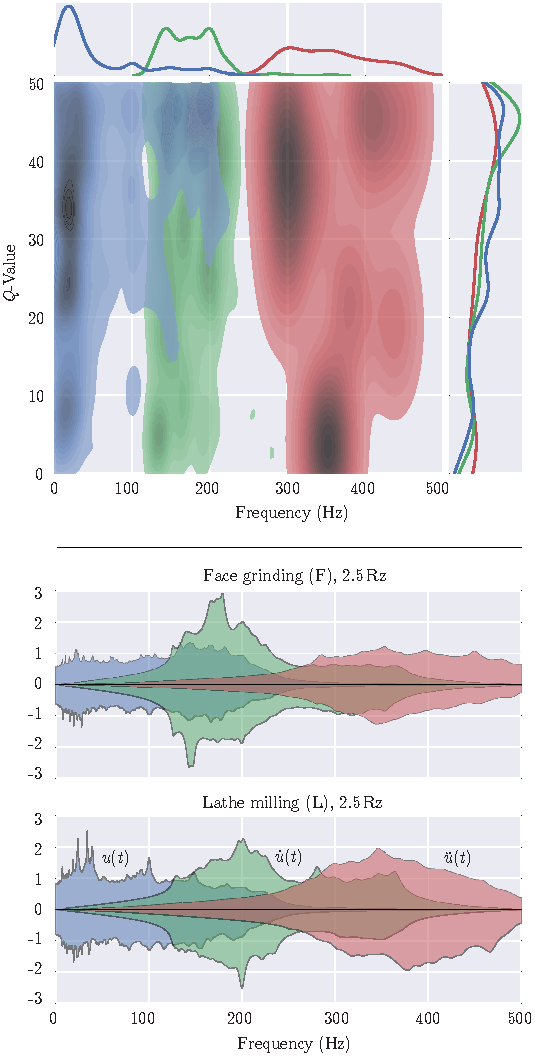
\includegraphics[width=0.4\textwidth]{touch-5}    
    \caption{\label{fig:touch-filters} Visualizing the network in the frequency domain. Frequencies are $0 - 250$, $125 - 375$, or $250 - 500$\,Hz, depending on whether each hidden neuron is encoding a dimension from $u(t)$ (blue), $\dot{u}(t)$ (green), or $\ddot{u}(t)$ (red). (Top) Distribution of bandpass filter parameters from (\ref{eq-bandpass}), weighted by the $\ell^2$-norm of SVM coefficients, and smoothed by a kernel density estimate \cite{michael_waskom_2015_19108}. 
The smallest weights are omitted to reduce visual clutter. Histograms along the sides flatten the distribution across their corresponding axes. (Bottom) Power of bandpass filters per texture (only two shown), weighted by their squared SVM coefficients (unitless). Negatively rectified dimensions are flipped about the $x$-axis for visualization.}
\end{figure}

To evaluate the system, the trained network was tested on each $1$\,s of test data. The 18-dimensional score vector was decoded from the spiking activity of the output population, lowpass filtered with default time constant ($5$\,ms), and sampled every $1$\,ms (see Fig. \ref{fig:touch-raster}). A total score for each texture was obtained by summing together the individual score vectors across the test segment. The classification for each test segment was taken to be the texture with the highest total score. These results are broken down by texture in Table \ref{tab:touch-results}, averaged across each test segment from all four folds, with an overall accuracy of $65.6\%$. The most common classification is the correct texture, in all cases.

By analyzing the trained network, we may succinctly characterize what each classifier is sensitive to in the frequency domain. We visualize this to indicate which bandpass parameters are most important for classifying all textures (see Fig. \ref{fig:touch-filters} top), and which frequencies are most important for classifying a specific texture (see Fig. \ref{fig:touch-filters} bottom). 
The top figure reveals that narrow filters (higher values of $Q$) tend to carry more weight, while frequencies in the range of $50 - 100$, $240 - 260$, and $400 - 500$\,Hz are less useful. The bottom figure shows for example that neurons encoding the negatively rectified dimension of $\dot{u}(t)$ will provide the most evidence for L2.5 when this dimension has power at $200$\,Hz. 

We also compared our approach to a simpler model, 
by training and evaluating the same model without a hidden layer. This baseline model was prepared and validated under the same conditions, except the SVM used the spiking activity of the mechanoreceptor population as its features, rather than the spiking activity from the hidden layer.  Cross-validation accuracy decreased to $17.8\%$, averaged across each test segment from all four folds.
We remark that the baseline still captures temporal information through its various lowpass filters (in the output layer and PSCs) and highpass filters (in the mechanoreceptor cells), yet it is no longer able to isolate particular bands of frequencies. Therefore, it is the addition of bandpass filters in the hidden layer that enable the network to accurately separate the feature space by texture.

\subsubsection{Discussion}

We trained a three-layer network of spiking neurons to classify a set of 18 textures. A biologically plausible model of mechanoreceptors was adapted to encode the input vibrations. Psychophysical experiments and the role of cuneate neurons motivated a hidden layer that extracts frequency information. Lastly, an SVM determined the connection weights into a recurrently connected population. To our knowledge this is a novel semi-supervised approach for classifying dynamic stimuli using a spiking neural network.

A key advantage of our approach is that the network can be simulated in real-time using low-power neuromorphic hardware. At the same time, the NEF endows our model with benefits such as robustness to noise  and parallel computation. Similarly, the system immediately provides classifications online, and performs well with brief inputs lasting only $1$\,s.  These advantages make our method generally suitable for use in robotic applications, thus advancing the state of the art for texture classification. % be more explicit? examples?

A comparison with a baseline model revealed that performance was a consequence of the hidden layer. The first two layers of the network are unsupervised, and so the activity of the hidden layer represents general features that can in theory be reused for other applications. We intend to demonstrate this by extending our system to differentiate between textures, by interpreting the feature vector as a high-dimensional description of a texture. We also suspect that other tasks which process tactile stimuli  can benefit by using this same vector.

Likewise, features of the input stimulus are learned and classified using general techniques from signal processing and machine learning. The methodology that we have described here need not be limited to the use of mechanoreceptor models and bandpass filters. While these tools were needed to appropriately constrain our model, other applications involving the processing of dynamic stimuli (e.g. visual or auditory) may readily place different constraints on how each layer encodes and filters information. This in turn may allow the architecture to be modified and redeployed within other domains. 

The test results indicate how often each texture is confused with another. 
In general, it should be possible to design a simple psychophysical experiment to compare our system to human performance. However, our system is at a fundamental disadvantage since it does not  alter its position or pressure to gather more evidence when unsure of its prediction. We are considering future extensions that solve this issue with a closed-loop system that can actively control its motor movements, with a range of velocities,  based on feedback from the accumulated features.

\subsection{Decoding Filter Optimization}

Include method of simultaneously solving for decoders and linear filter in a single least-squares problem

\subsection{Dale's Principle}

Compare my DalesSolver to Parisian Transform


\section{Biological Detail}

\subsection{Conductance-Based Synapses}

Summarize Andreas' research

\subsection{Adaptative Neurons}

Eric's system itendification
Subtractive adaptation and perfect cancellation
Divisive adaptation (adaptive threshold) and modelling it by the latter
Interpretation in terms of PSC code / objective function, and dimensionality

\subsection{Wilson Neurons}

Peter's work

\subsection{Baal Neurons}

Peter's work



\chapter{Delay Networks}
\label{chapt:delays}

This section is taken from \citet{voelker2018}.

A fundamental dynamical system that has not yet been discussed within the NEF literature is the continuous-time delay line of $\theta$ seconds,\footnote{
\citet{voelker2015computing} proposed a NEF model, but did not include detailed analysis or extensions.
% Here, we elaborate on this network in considerable detail.
}
expressed as:
\begin{align} \label{eq:time-delay}
y(t) = (u \ast \delta_{-\theta})(t) = u(t - \theta)\text{,} \quad \theta > 0 \text{,}
\end{align}
where $\delta_{-\theta}$ denotes a Dirac delta function shifted backwards in time by $\theta$.
This system takes a time-varying scalar signal, $u(t)$, and outputs a purely delayed version, $u(t - \theta)$.
The task of computing this function both accurately and efficiently in a biologically plausible, spiking, dynamical network, is a significant theoretical challenge, that, to our knowledge, has previously remained unsolved.

The continuous-time delay is worthy of detailed consideration for several reasons.
First, it is non-trivial to implement using continuous-time spiking dynamical primitives.
Specifically, equation~\ref{eq:time-delay} requires that we maintain a \emph{rolling window} of length $\theta$ (i.e.,~the history of $u(t)$, going $\theta$ seconds back in time).
Thus computing a delay of $\theta$ seconds is just as hard as computing every delay of length $\theta'$, for all $0 \le \theta' \le \theta$.
Since any finite interval of $\mathbb{R}$ contains an uncountably-infinite number of points, an exact solution for arbitrary $u(t)$ requires that we maintain an uncountably-infinite amount of information in memory.
Second, the delay provides us with a window of input history from which to compute arbitrary nonlinear functions across time.
For instance, the spectrogram of a signal may be computed by a nonlinear combination of delays, as may any finite impulse response~(FIR) filter.
Third, delays introduce a rich set of interesting dynamics into large-scale neural models, including: oscillatory bumps, traveling waves, lurching waves, standing waves, aperiodic regimes, and regimes of multistability~\citep{roxin2005role}.
Fourth, a delay line can be coupled with a single nonlinearity to construct a network displaying many of the same benefits as Reservoir Computing~\citep{appeltant2011information}.
Finally, examining the specific case of the continuous-time delay introduces several methods and concepts we employ in generally extending the NEF (section~\ref{sec:extensions}).

\TODO{Takens Theorem}

\section{Conventional Approaches}

Reservoir computing / FORCE / LSTMs?
\TODO{Discuss "Reservoir Computing Beyond Memory-Nonlinearty Trade-off Inubushi \& Yoshimura, and Information Processing Capacity of Dynamical Systems Massar et al.}

\section{Optimal NEF Solution}
\label{sec:nef-delay}

As it is impossible in practice (i.e.,~given finite-order continuous-time resources) to implement an arbitrary delay, we will instead approximate $u(t)$ as a low-frequency signal, or, equivalently, approximate equation~\ref{eq:time-delay} as a low-dimensional system expanded about the zeroth frequency in the \emph{Laplace domain}.
We begin by transforming equation~\ref{eq:time-delay} into the Laplace domain, $\mathcal{L} \left\{ y(t) \right\} = \mathcal{L} \left\{ u(t) \right\} \mathcal{L} \left\{ \delta_{-\theta}(t) \right\}$, and then using the fact that $\mathcal{L} \left\{ \delta_{-\theta}(t) \right\} = e^{-\theta s}$ to obtain:
\begin{align} \label{eq:tf-delay}
F(s) := \frac{\mathcal{L} \left\{ y(t) \right\}}{\mathcal{L} \left\{ u(t) \right\}} = e^{-\theta s} \text{,}
\end{align}
where $F(s)$ is known as the \emph{transfer function} of the system, defined as the ratio of the Laplace transform of the output to the Laplace transform of the input.
Equation~\ref{eq:tf-delay} should be understood as an equivalent way of expressing equation~\ref{eq:time-delay} in the Laplace domain, where the variable $s$ denotes a complex frequency. 
Thus far, we have only described the transfer function that we would like the network to implement. %while $t$ is non-negative in the time domain.
% Unimportant reminder? The transfer function is the Laplace transform of system's impulse response.

The state-space model discussed in section~\ref{sec:principle3} (equation~\ref{eq:lti}) is related to its transfer function by the following:
\begin{align} \label{eq:ss2tf}
F(s) = C(sI - A)^{-1}B + D \text{.}
\end{align}
Conversely, a transfer function can be converted into a state-space model satisfying equation~\ref{eq:ss2tf} \emph{if and only if} it can be written as a proper ratio of finite polynomials in $s$~\citep{brogan1982modern}.
The ratio is proper when the degree of the numerator does not exceed that of the denominator.
In such a case, the output will not depend on future input, and so the system is \emph{causal}.
The degree of the denominator corresponds to the dimensionality of the state-vector, and therefore must be finite.
These two conditions align with physically realistic constraints where time may only progress forward, and neural resources are limited.

However, the pure delay (equation~\ref{eq:tf-delay}) has infinite order when expressed as a ratio of polynomials in $s$, and so the system is irrational, or infinite-dimensional.
Consequently, no finite state-space model will exist for $F(s)$, which formalizes our previous intuition that an exact solution is impossible for finite, continuous-time systems.
To overcome this, we must approximate the irrational transfer function $e^{-\theta s}$ as a proper ratio of finite-order polynomials.
We do so using its \emph{Pad\'e approximants}---the coefficients of a Taylor series extended to the ratio of two polynomials---expanded about $s=0$~\citep{Pade1892, vajta2000some}:
\begin{equation} \label{eq:pade}
\begin{aligned}
\left[ p/q \right] e^{-\theta s} &= \frac{\mathcal{B}_{p}(-\theta s)}{\mathcal{B}_{q}(\theta s)} \text{,} \\
\quad \mathcal{B}_m(s) &:= \sum_{i=0}^m \begin{pmatrix}m \\ i\end{pmatrix} \frac{(p + q - i)!}{(p + q)!} s^i \text{.}
\end{aligned}
\end{equation}
This provides the transfer function of order $p$ in the numerator and order $q$ in the denominator that optimally approximates equation~\ref{eq:tf-delay} for low-frequency inputs (i.e.,~up to order $p + q$).

After choosing $0 \le p \le q$, we may numerically find a state-space model $(A\text{,}\, B\text{,}\, C\text{,}\, D)$ that satisfies equation~\ref{eq:ss2tf} using standard methods,\footnote{
For instance, the function \texttt{tf2ss} in MATLAB or SciPy.}
and then map this system onto the synapse using Principle~3.
%This works independently of the chosen simulation time-step using equation~\ref{eq:p3discrete}.
However, na\"ively applying this conversion leads to numerical issues in the representation (i.e.,~dimensions that grow exponentially in magnitude), due in part to the factorials in equation~\ref{eq:pade}.

To overcome this problem, we derive an equivalent yet normalized state-space model that we have not encountered elsewhere.
We do so for the case of $p = q - 1$, since this provides the best approximation to the step-response. We symbolically transform equation~\ref{eq:pade} into a normalized state-space model that avoids the need to compute any factorials.
We first do so for the special case of $p = q - 1$, since this provides the best approximation to the step-response~\citep{vajta2000some}.
We begin by expanding equation~\ref{eq:pade}:
\begin{align*}
[q-1/q]e^{-\theta s} &= \frac{\sum_{i=0}^{q-1} \begin{pmatrix}{q-1} \\ i\end{pmatrix} (2q - 1 - i)! (-1)^i \theta^i s^i}{\sum_{i=0}^q \begin{pmatrix}q \\ i\end{pmatrix} (2q - 1 - i)! \theta^i s^i} \\
&= \frac{\frac{1}{\theta^{q} (q-1)!} \sum_{i=0}^{q-1} \frac{(q-1)!}{(q-1-i)!i!} (2q - 1- i)! \theta^i s^i (-1)^i}{s^q + \frac{1}{\theta^q (q-1)!}  \sum_{i=0}^{q-1} \frac{q!}{(q-i)!i!} (2q - 1 - i)! \theta^i s^i} \\
&= \frac{\sum_{i=0}^{q-1} c_i s^i}{s^q + \sum_{i=0}^{q-1} d_i s^i} \text{,}
\end{align*}
where $d_i := \frac{q(2q - 1 - i)!}{(q-i)!i!} \theta^{i-q}$ and $c_i := (-1)^i \left( \frac{q-i}{q} \right) d_i$.

This transfer function is readily converted into a state-space model in controllable canonical form:
\begin{equation*}
    \begin{alignedat}{2}
        A &= \begin{pmatrix} -d_{q-1} & -d_{q-2} & \cdots & -d_0 \\ 1 & 0 & \cdots & 0 \\ 0 & \ddots & \ddots & \vdots \\ 0 & 0 & 1 & 0\end{pmatrix} \text{,} & & \quad\quad \begin{alignedat}{1}
            B &= \transpose{\begin{pmatrix} 1 & 0 & \cdots & 0\end{pmatrix}} \text{,} \\
            C &= \begin{pmatrix} c_{q-1} & c_{q-2} & \cdots & c_0\end{pmatrix} \text{,} \\
            D &= 0 \text{.}
        \end{alignedat}
    \end{alignedat}
\end{equation*}

To eliminate the factorials in $d_i$ and $c_i$, we scale the $i^{\text{th}}$ dimension of the state-vector by $d_{q-1-i}$, for all $i = 0 \ldots q - 1$.
This is achieved without changing the transfer function by scaling each $(B)_j$ by $d_{q-1-j}$, each $(C)_i$ by $1 / d_{q-1-i}$, and each $(A)_{ij}$ by $d_{q-1-i} / d_{q-1-j}$, which yields the equivalent state-space model:
\begin{equation}
    \begin{alignedat}{2}
        A &= \begin{pmatrix} -v_0 & -v_0 & \cdots & -v_0 \\ v_1 & 0 & \cdots & 0 \\ 0 & \ddots & \ddots & \vdots \\ 0 & 0 & v_{q-1} & 0\end{pmatrix} \text{,} & & \quad\quad \begin{alignedat}{1}
            B &= \transpose{\begin{pmatrix} v_0 & 0 & \cdots & 0\end{pmatrix}} \text{,} \\
            C &= \begin{pmatrix} w_0 & w_1 & \cdots & w_{q-1} \end{pmatrix} \text{,} \\
            D &= 0 \text{,} \label{eq:ss-delay}
        \end{alignedat}
    \end{alignedat}
\end{equation}
where $v_i := \frac{(q+i)(q-i)}{i+1} \theta^{-1}$ and $w_i := (-1)^{q - 1 - i} \left( \frac{i+1}{q} \right)$, for $i = 0 \ldots q-1$.
This follows from noting that $v_0 = d_{q-1}$ and $v_i := d_{q-1-i} / d_{q-i}$ for $i \ge 1$.

A similar derivation applies to the case where $p = q$, although it results in a passthrough ($D \ne 0$) which is suboptimal for step-responses.
For brevity, we omit this derivation, and instead simply state the result:
\begin{equation*}
    \begin{alignedat}{2}
        A &= \begin{pmatrix} -v_0 & -v_0 & \cdots & -v_0 \\ v_1 & 0 & \cdots & 0 \\ 0 & \ddots & \ddots & \vdots \\ 0 & 0 & v_{q-1} & 0\end{pmatrix} \text{,} & & \quad\quad \begin{alignedat}{1}
            B &= \transpose{\begin{pmatrix}-v_0 & 0 & \cdots & 0\end{pmatrix}} \text{,} \\
            C &= \begin{pmatrix} 2(-1)^q & 0 & 2(-1)^q & 0 & \cdots & \cdots \end{pmatrix} \text{,} \\
            D &= (-1)^q \text{,}
        \end{alignedat}
    \end{alignedat}
\end{equation*}
where $v_i = \frac{(q+i+1)(q-i)}{i+1} \theta^{-1}$, for $i = 0 \ldots q-1$.

In either case, $A$ and $B$ depend on the delay length solely by the scalar factor $\theta^{-1}$.
As a result, we may \emph{control} the length of the delay by adjusting the gain on the input and feedback signals.
The NEF can be used to build such controlled dynamical systems, without introducing multiplicative dendritic interactions or implausible on-the-fly connection weight scaling~\citep{eliasmith2000b}.
The identification of this control factor is connected to a more general property of the Laplace transform, $F \left( a^{-1} s \right) = \mathcal{L} \left\{ a f(at) \right\}$ for all $a > 0$, that we can exploit to modulate the width of any filter on-the-fly (in this case affecting the amount of delay; results not shown).

This model is now equivalent to equation~\ref{eq:pade}, but without any factorials, and in the form of equation~\ref{eq:lti}.\footnote{
In appendix~\ref{app:state-space}, we provide some additional manipulations of the state-space model.}
The choice of $q$ corresponds to the dimensionality of the latent state-vector $\V{x}(t)$ that is to be represented by Principle~1 and transformed by Principle~2.
Principle~3 may then be used to map equation~\ref{eq:ss-delay} onto a spiking dynamical network to accurately implement an optimal low-frequency approximation of the delay.

To demonstrate, we implement a $1$\,s delay of $1\,$Hz band-limited white noise using $\num{1000}$ recurrently connected spiking LIF neurons representing a $6$-dimensional vector space (see Figure~\ref{fig:delay-example}).
The connections between neurons are determined by applying Principle~3 (section~\ref{sec:principle3}) to the state-space model derived above (equation~\ref{eq:ss-delay}, $q=6$) via the Pad\'e approximants of the delay.
The normalized root-mean-squared error (NRMSE) of the output signal is $0.048$ (normalized so that $1.0$ would correspond to random chance).
This is achieved without appealing to the simulation time-step ($dt = 1$\,ms); in fact, as shown in section~\ref{sec:pure_delay}, the network accuracy improves as $dt$ approaches zero due to the continuous-time assumption mentioned in section~\ref{sec:principle3} (and resolved in section~\ref{sec:discrete-lowpass}).

\begin{figure}
  \centering
  \includegraphics[width=\textwidth]{{NECO-04-17-2838-Figure.3}.pdf}
  \caption{ \label{fig:delay-example}
    Delay of $1$\,s implemented by applying standard Principle~3 to equation~\ref{eq:ss-delay} using $q = 6$, $dt=1$\,ms, $\num{1000}$ spiking LIF neurons, and a lowpass synapse with $\tau=0.1$\,s.
    The input signal is white noise with a cutoff frequency of $1$\,Hz.
    The plotted spikes are filtered with the same $\tau=0.1$\,s, and encoded with respect to $\num{1000}$ encoders sampled uniformly from the surface of the hypersphere (sorted by time to peak activation).
  }
\end{figure}

Although the delay network has its dynamics optimized for a single delay $\theta > 0$, we can still accurately decode any delay $0 \le \theta' \le \theta$ from the same network.
This means that the network is representing a rolling window (i.e.,~history) of length $\theta$.
This window forms a temporal code of the input stimulus.

To compute these other delays, we would like to optimally approximate $e^{-\theta' s}$ with a transfer function $F_{\theta \rightarrow \theta'}(s) := \frac{\mathcal{C}(s; \, \theta, \theta')}{\mathcal{D}(s; \, \theta)}$ of order $[p / q]$, such that the denominator $\mathcal{D}(s; \, \theta)$ (which provides us with the recurrent transformation up to a change of basis) depends only on $\theta$, while the numerator $\mathcal{C}(s; \, \theta, \theta')$ (which provides us with the output transformation up to a change of basis) depends on some relationship between $\theta'$ and $\theta$.

From equation~\ref{eq:pade}, we may write the denominator as:
\begin{align*}
\mathcal{D}(s; \, \theta) = \sum_{i=0}^q d_i(\theta) s^i \text{,} \quad d_i(\theta) := \begin{pmatrix}q \\ i\end{pmatrix} \frac{(p + q - i)!}{(p + q)!} \theta^i \text{.}
\end{align*}
We then solve for the numerator, as follows:
\begin{align*}
&& [p/q] e^{-\theta' s} &= \sum_{i=0}^\infty \frac{(-\theta' s)^i}{i !} = \frac{\mathcal{C}(s; \, \theta, \theta')}{\mathcal{D}(s; \, \theta)} & \\
&& \iff \quad \mathcal{C}(s; \, \theta, \theta') &= \left( \sum_{i=0}^\infty \frac{(-\theta' s)^i}{i !} \right) \left( \sum_{j=0}^q d_j(\theta) s^j \right) + \bigoh{s^{p + 1}} \text{.}
\end{align*}
By expanding this product and collecting like terms, the correct numerator up to order $p \le q$ is:
\begin{align*}
\mathcal{C}(s; \, \theta, \theta') = \sum_{i=0}^p c_i(\theta, \theta') s^i \text{,} \quad c_i(\theta, \theta') :=  \sum_{j=0}^i \frac{(- \theta')^{i - j}}{(i - j)!} d_j(\theta) \text{.}
\end{align*}
Therefore, the optimal readout for a delay of length $\theta'$, given the dynamics for a delay of length $\theta$, is determined by the above linear transformation of the coefficients $\left( d_j(\theta) \right)_{j=0}^p$.

We remark that $c_i(\theta, \theta) = \begin{pmatrix}p \\ i\end{pmatrix} \frac{(p + q - i)!}{(p + q)!} (-\theta)^i$, since $F_{\theta \rightarrow \theta}(s) = [p/q] e^{-\theta s}$, by uniqueness of the Pad\'e approximants, and by equation~\ref{eq:pade}.
As a corollary, we have proven that the following combinatorial identity holds for all $p, q \in \mathbb{N}$ and $i \in \left[ 0, \min\{p, q\} \right]$:
\begin{align*}
\begin{pmatrix}p \\ i\end{pmatrix} = \sum_{j=0}^i (-1)^j \begin{pmatrix}q \\ j\end{pmatrix} \begin{pmatrix}p + q - j \\ i - j\end{pmatrix} \text{.}
\end{align*}

For the case when $p = q - 1$, we may also apply the same state-space transformation from appendix~\ref{app:ss-delay} to obtain the normalized coefficients for the $C$ transformation (i.e.,~with $A$, $B$, and $D$ from equation~\ref{eq:ss-delay}):
\begin{align*}
w_{q-1-i} &= \left( \sum_{j=0}^i \frac{(-\theta')^{i-j}}{(i - j)!} \begin{pmatrix}q \\ j\end{pmatrix} \frac{(2q - 1 - j)!}{(2q - 1)!} \theta^j \right) \left( \frac{(q - i)! i! (2q - 1)!}{\theta^q (q - 1)! q(2q - 1 - i)!} \theta^{q - i} \right) \\
&= \sum_{j=0}^i \begin{pmatrix}q \\ j\end{pmatrix} \left( \frac{(2q - 1 - j)!}{(i - j)! (2q - 1 - i)!} \right) \left( \frac{(q - i)! i!}{q!} \right) \left( \theta^{j - i} \right) (-\theta')^{i - j} \\
&= \begin{pmatrix}q \\ i\end{pmatrix}^{-1} \sum_{j=0}^i \begin{pmatrix}q \\ j\end{pmatrix} \begin{pmatrix}2q - 1 - j \\ i - j\end{pmatrix} \left( \frac{-\theta'}{\theta} \right)^{i - j} \text{,} \quad i = 0 \ldots q - 1 \text{.}
\end{align*}

The $q$-dimensional state-vector of the delay network represents a rolling window of length $\theta$.
That is, a single delay network with some fixed $\theta > 0$ may be used to accurately decode any delay of length $\theta'$ ($0 \le \theta' \le \theta$).
Different decodings require different linear output transformations ($C$) for each $\theta'$, with the following coefficients:
\begin{align} \label{eq:delay-readouts}
w_{q-1-i} = \begin{pmatrix}q \\ i\end{pmatrix}^{-1} \sum_{j=0}^i \begin{pmatrix}q \\ j\end{pmatrix} \begin{pmatrix}2q - 1 - j \\ i - j\end{pmatrix} \left( \frac{-\theta'}{\theta} \right)^{i - j} \text{,} \quad i = 0 \ldots q - 1 \text{.} 
\end{align}
The underlying dynamical state remains the same.

% Apart from providing a means of understanding the state-vector, the basis functions from equation~\ref{eq:delay-readouts} also provide a number of ways to readily exploit the delay network.
% a) differentiate any point up to q times
% b) "preferred window" of each neuron
% c) projecting the window function onto state-space
% d) characterizing the possible functions using Principles 1+2 and the inverse basis functions

In Figure~\ref{fig:delay-full}, we take different linear transformations of the same state-vector, by evaluating equation~\ref{eq:delay-readouts} at various delays between $0$ and $\theta$, to decode the rolling window of input from the state of the system.\footnote{
The optimization problem from equation~\ref{eq:decoder_solution} need only be solved once to decode $\V{x}(t)$ from the neural activity.
The same decoders may then be transformed by each $C$ without loss in optimality (by linearity).
}
This demonstrates that the delay network compresses the input's history (lasting $\theta$ seconds) into a low-dimensional state.

\begin{figure}
  \centering
  \includegraphics[width=\textwidth]{{NECO-04-17-2838-Figure.4}.pdf}
  \caption{ \label{fig:delay-full}
    Decoding a rolling window of length $\theta$.
    Each line corresponds to a different delay, ranging from $0$ to $\theta$, decoded from a single delay network ($q = 12$).
    (Left)~Error of each delay, as the input frequency is increased relative to $\theta$.
    Shorter delays are decoded more accurately than longer delays at higher frequencies.
    A triangle marks $\theta = \text{Frequency}^{-1}$.
    (Right)~Example simulation decoding a rolling window of white noise with a cutoff frequency of $\theta^{-1}$\,Hz.
    % See appendix~\ref{app:window} for details.
  }
\end{figure}

In Figure~\ref{fig:basis-functions}, we sweep equation~\ref{eq:delay-readouts} across $\frac{\theta'}{\theta}$ to visualize the temporal ``basis functions'' of the delay network.
This provides a way to understand the relationship between the chosen state-space representation (i.e.,~the $q$-dimensional $\V{x}(t)$) and the underlying window representation (i.e.,~the infinite-dimensional $u(t)$).
In particular, each basis function corresponds to the continuous window of history represented by a single dimension of the delay network.
The instantaneous value of each dimension acts as a coefficient on its basis function, to contribute to the representation of the window at that point in time.
Overall, the entire state-vector determines a linear combination of these $q$ basis functions to represent the window.
This is analogous to the static function representation explored previously within the context of Principles~1 and~2~\citep[][pp.~63--72]{eliasmith2003a}.

\begin{figure}
  \centering
  \includegraphics[width=\textwidth]{{NECO-04-17-2838-Figure.5}.pdf}
  \caption{ \label{fig:basis-functions}
    Temporal basis functions of the delay network ($q = 12$).
    Each line corresponds to the basis function of a single dimension~($i$) ranging from $0$~(darkest) to $q - 1$~(lightest).
    The $i^\text{th}$ basis function is a polynomial over $\frac{\theta'}{\theta}$ with degree $i$ (see equation~\ref{eq:delay-readouts}). % ($0 \le \theta' \le \theta$).
    The state-vector of the delay network takes a linear combination of these $q$ basis functions in order to represent a rolling window of length $\theta$.
  }
\end{figure}

The encoder of each neuron can also be understood directly in these terms as taking a linear combination of the basis functions (via equation~\ref{eq:encoding}).
Each neuron nonlinearly encodes a projection of the rolling window onto some ``preferred window'' determined by its own encoder.
Since the state-vector is encoded by heterogeneous neural nonlinearities, the population's spiking activity supports the decoding of nonlinear functions across the entire window (i.e.,~functions that we can compute using Principles~1 and~2).
Therefore, we may conceptualize the delay network as a \emph{temporal coding} of the input stimulus, which constructs a low-dimensional state---representing an entire window of history---to encode the temporal structure of the stimulus into a nonlinear high-dimensional space of neural activities.

To more thoroughly characterize the delay dynamics, we analyze the behavior of the delay network as the dimensionality is increased (see Figure~\ref{fig:pca}).
Specifically, we perform a standard principal component analysis~(PCA) on the state-vector for the impulse response, and vary the order from $q=3$ to $q=27$.
This allows us to visualize a subset of the state-vector trajectories, via projection onto their first three principal components (see Figure~\ref{fig:pca}-Top). %\footnote{
%These same trajectories are obtained by a PCA on the %filtered neural activities, by linearity of decoding.
%}
The length of this trajectory over time distinguishes different values of $q$ (see Figure~\ref{fig:pca}-Bottom).
This length-curve is approximately logarithmic when $q = 6$, convex when $q \le 12$, and sigmoidal when $q > 12$. % (also see Figure~\ref{fig:time-cells}-Bottom).
To generate this figure we use a delay of $\theta = 10\,$s, but in fact this analysis is scale-invariant with time.
This means that other delays will simply stretch or compress the impulse response linearly in time (not shown).

\begin{figure}
  \centering
  \includegraphics[width=\textwidth]{{NECO-04-17-2838-Figure.6}.pdf}
  \caption{ \label{fig:pca}
    Impulse response of the delay network with various orders ($q$) of Pad\'e approximants.
    (Top)~The state-vector $\V{x}(t)$ projected onto its first three principal components.
    (Bottom)~The length of the curve $\V{x}$ up to time $t$, computed using the integral $\int_0^t \|\dot{\V{x}}(t')\| \, dt'$ (normalized to $1$ at $t = \theta$).
    This corresponds to the distance travelled by the state-vector over time.
    The dashed line marks the last inflection point, indicating when $\V{x}(t)$ begins to slow down.
    % The slope of $d(t)$ is correlated with the number of neurons encoding $\V{x}(t)$ at time $t$, when using a random encoding (not shown).
  }
\end{figure}

We remark that the delay network is scale-invariant with the delay length over input frequency, that is, the accuracy for a chosen order is a function of $s \times \theta$ (see units in Figure~\ref{fig:delay-full} for instance). % and the synaptic time-constants are scaled by $\theta$.
More specifically, for a fixed approximation error, the delay length scales as $\bigoh{ \frac{q}{f} }$, where $f$ is the input frequency.
Then, the accuracy of the mapped delay is a function of the relative magnitude of the delay length to $\frac{q}{f}$, whose exact shape depends on the considered synapse model.
To determine these functions for a wide class of synapses, we proceed by extending the NEF.

\section{Computational Properties}

\subsection{Nonlinear Characterization}

We present a dynamical system that optimally compresses a rolling time window of input into a low-dimensional state-space.
The state of this system represents the history of its input by a linear combination of time-invariant polynomial basis functions.
We use the Neural Engineering Framework~(NEF) to compile this system onto a recurrent spiking neural network.
The activity of this ``delay network'' naturally approximates a Taylor series expansion, over time, centered about every point within the window.
We show that this permits the computation of arbitrary nonlinear computations across the history of an input stimulus, while outperforming Echo State Networks in accuracy and training/testing time, without explicitly simulating any training examples.

A continuous-time rolling window of length $\theta > 0$, denoted $[ u(t - \theta') \,:\, 0 \le \theta' \le \theta ]$, may be \emph{temporally compressed} into a low-dimensional state $\V{x}(t) \in \mathbb{R}^d$, by the following linear time-invariant dynamical system that approximately delays an input signal by $\theta$ seconds~\citep{voelker2018}:
\begin{equation} \label{eq:delay-system}
  \dot{\V{x}}(t) = A\V{x}(t) + Bu(t) \text{,} \quad
  A = \begin{pmatrix} -v_0 & -v_0 & \cdots & -v_0 \\ v_1 & 0 & \cdots & 0 \\ 0 & \ddots & \ddots & \vdots \\ 0 & 0 & v_{d-1} & 0\end{pmatrix} \text{,} \quad 
  B = \transpose{\begin{pmatrix} v_0 & 0 & \cdots & 0\end{pmatrix}} \text{,} 
\end{equation}
where $v_i := \frac{(d+i)(d-i)}{i+1} \theta^{-1}$, %and $w_i := (-1)^{d - 1 - i} \left( \frac{i+1}{d} \right)$
for $i = 0 \ldots d-1$.
%We may also solve this system to express $\V{x}(t)$ as a convolution of $u$ with the SIMO impulse response $\V{f}$: 
%\begin{equation} \label{eq:lti-solved}
%\V{f}(t) = e^{At} B \text{,} \quad \V{x}(t) = \left(u \ast \V{f}\right)(t) \text{.}
%\end{equation}
This compression is derived by applying Pad\'e approximants to $e^{-\theta s}$ about the complex point $s=0$, which yields an optimal low-degree polynomial expansion of $\mathcal{L}\{u\}(s)$ about its zeroth frequency.
%\footnote{Note that a LTI system is equivalent up to any invertible linear transformation applied to the state-space.}
The state $\V{x}(t)$ represents the rolling window via a linear combination of time-invariant polynomial basis functions:
\begin{equation} \label{eq:basis-interpretation}
\boxed{u(t - \theta') \approx \sum_{i=0}^{d-1} \mathcal{P}_{i,d} \left(\frac{\theta'}{\theta} \right) \, x_{d-1-i}(t) \text{,} \quad 0 \le \theta' \le \theta \text{,}}
\end{equation}
which we have solved in closed-form~\citep[][eq.~14]{voelker2018}:
\begin{equation} \label{eq:basis-functions}
\mathcal{P}_{i,d}(r) = \begin{pmatrix}d \\ i\end{pmatrix}^{-1} \sum_{j=0}^i \begin{pmatrix}d \\ j\end{pmatrix} \begin{pmatrix}2d - 1 - j \\ i - j\end{pmatrix} \left( -r \right)^{i - j} \text{.} %\text{,}\quad 0 \le r \le 1 \text{,}\quad i = 0 \ldots d - 1
\end{equation}
A set of polynomials $\{ \mathcal{P}_{i, d} \}$ are shown in Figure~\ref{fig:basis-functions}.
This defines a linear map from the $d$-dimensional state, $\V{x}(t)$, to the infinite-dimensional rolling window, $[ u(t - \theta') \,:\, 0 \le \theta' \le \theta ]$.
In other words, (\ref{eq:basis-interpretation}) is the optimal pseudoinverse of the linear compression defined by (\ref{eq:delay-system}).
%The frequencies in $u(t)$ that may be accurately encoded by this approach scale inversely with $\theta$.
%Likewise, higher values of $q$ allowed for higher frequencies to be encoded at the same level of precision.
%We remark that each basis function is expressed in terms of the unitless quantity $\frac{\theta'}{\theta}$, and is therefore scale-invariant.
%We may also transform the state by any invertible matrix (e.g.,~ to orthogonalize the basis functions) without loss of generality.
%Analysis of the approximation error, and some additional properties of this ``delay network'', may be found in \cite{voelker2018}.
Moreover, each point along the window, along with its Taylor series expansion up to order $d-1$, as well as any other linear operation across the rolling window (e.g.,~Laplace transform), may be expressed using (\ref{eq:basis-interpretation}) and (\ref{eq:basis-functions}) as a known dot-product with $\V{x}(t)$.
%Yet, as shown below, this does not restrict our ability to also perform nonlinear computations across the window.

\begin{figure}
\centering
  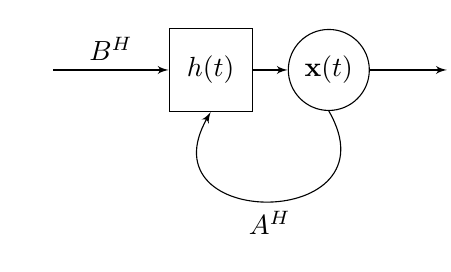
\begin{tikzpicture}[auto, >=latex']
    \node [input] (u) {$u(t)$};
    \node [block, right of=u, node distance=2cm] (h) {$h(t)$};
    \node [ensemble, right of=h, node distance=1.5cm] (x) {$\V{x}(t)$};
    \node [output, right of=x, node distance=1.5cm] (y) {$y(t)$};
    \draw [->] (u) -- node {$B^H$} (h);
    \draw [->] (h) -- (x);
    %\draw [->] (x.north) -- (y);
    \draw [->] (x) -- (y);
    %\draw [->] (x.south) -- (y);
    \path[->] (x.south) edge [loop below, min distance=5em, out=-60, in=-120] node {$A^H$} (h.south);
  \end{tikzpicture}
  \caption{ \label{fig:delay-architecture}
    Delay network~(DN) architecture.
    The synapse model $h(t)$ is driven by $A^H \V{x}(t) + B^H u(t)$ to yield the state $\V{x}(t)$. 
    This state is nonlinearly encoded by a heterogeneous population of neurons and subsequently decoded to estimate the desired $y(t)$.
  } 
\end{figure}

\begin{figure}
\centering
  \includegraphics[width=0.5\linewidth]{delay-autocorrelation}
  \caption{ \label{fig:delay-autocorrelation} 
    Visualizing the autocorrelation function $y(t) = u(t - \theta)\, u(t)$ with $d=3$.
    Each point along the surface of the unit-sphere is $\V{x}(t)$, and is colored according to its corresponding value of $y(t)$ obtained from (\ref{eq:basis-interpretation}).
    A slice of the shell is cut away for visualization.
  } 
\end{figure}

To implement this system as a recurrent neural network, we use the Neural Engineering Framework~\citep[NEF;][]{eliasmith2003a} to map (\ref{eq:delay-system}) onto the dynamics of a lowpass synapse with time-constant $\tau$:
\begin{equation}
A^H = \tau A + I \text{,} \quad B^H = \tau B \text{,} \quad H(s) = \left(\tau s + 1\right)^{-1} \text{.}
\end{equation}
The resulting ``delay network''~(DN) is depicted in Figure~\ref{fig:delay-architecture}.
Generalizations to arbitrary linear synapses, including those modelling pure feedback delays, may be found in %\cite{voelker2017b}.
\cite{voelker2018}.
The state $\V{x}(t)$ is \emph{encoded} by a heterogeneous population of neurons, which allows arbitrary nonlinear functions across the window, $y(t) = f(\V{x}(t))$, to be \emph{decoded} from its activity~\citep{eliasmith2003a}.

\subsection{Scalability}
\label{sec:delay-scalability}

\TODO{stress that the state for one delay is the same for another with a stretched input}

\TODO{error plots for pade\_delay\_error from nengolib and talk about multiple layers}

In section~\ref{sec:deep-delay-networks} we discuss the scaling properties of multiple DNs stacked together to form a Deep Delay Network~(DDN).

\section{Applications}
\label{sec:delay-applications}

\TODO{write} Linear and nonlinear window computation. Computational neural modelling.

\subsection{Optimized Reservoir Computing}

RC networks often include a sparsity constraint of $20\%$ connectivity, which is still $\bigoh{n^2}$, in order to improve accuracy~\citep{lukovsevicius2012reservoir}.
We also considered ESNs with constant sparsity~\citep{lukovsevivcius2012practical}, similar to our NEF networks, but found that they did not perform comparably to our results in section~\ref{sec:delay_benchmark}.

Constructing a network to implement a delay is a natural way to measure the network's ability to maintain a history of its input signal, which is needed to compute any function over past inputs.
Indeed, this task was considered by ESNs in one of the earliest demonstrations of the RC paradigm~\citep{jaeger2002short}.  In its purest form, the delay network (DN) is attempting to encode an infinite amount of information, which is why it is a challenging and useful benchmark to consider.

For the benchmark tasks, weights were trained and validated using randomly sampled band-limited white noise.
In addition, full-spectrum white-noise was added to the network during both training and testing.
Accuracy was measured by normalizing the root-mean squared error against the root-mean squared target~\citep[NRMSE;][]{lukovsevicius2012reservoir}.
As well, $95\%$ confidence intervals were bootstrapped and plotted using Seaborn~\citep{michael_waskom_2015_19108}.
The free parameters for each method were optimized using $200$ iterations of Hyperopt~\citep{bergstra2013making} with $3$ trials per iteration, to maximize the validation error for $200$\,ms delays (see Table~\ref{tab:hyperopt}).
LSMs were implemented by replacing the $\tanh$ units with LIF spiking neurons, making them comparable to our NEF networks but with full-rank weight matrices.
All data and figures may be reproduced by following the instructions at the following URL: \path{https://github.com/arvoelke/rc2017}.

\begin{table}\centering
  %\ra{1.2}
  \noindent\begin{tabularx}{\textwidth}{YYYYYY}
    \toprule
     & ESN & LSM & NEF with Rate LIF & NEF with Rate Tan & NEF with Spike LIF \\
    \midrule
Gain & \num[round-precision=3,round-mode=figures,scientific-notation=true]{1.3251896701} & \num[round-precision=3,round-mode=figures,scientific-notation=true]{0.00315170551016} &  &  &  \\

Radius & \num[round-precision=3,round-mode=figures,scientific-notation=true]{24.3145093319} & \num[round-precision=3,round-mode=figures,scientific-notation=true]{1.36259213791} & \num[round-precision=3,round-mode=figures,scientific-notation=true]{4.63655157006} & \num[round-precision=3,round-mode=figures,scientific-notation=true]{12.8794579757} & \num[round-precision=3,round-mode=figures,scientific-notation=true]{0.577484080063} \\

$\tau_\mathrm{readout}$ & \num[round-precision=3,round-mode=figures,scientific-notation=true]{0.00686793487811} & \num[round-precision=3,round-mode=figures,scientific-notation=true]{0.0604400629751} & \num[round-precision=3,round-mode=figures,scientific-notation=true]{0.0606008691858} & \num[round-precision=3,round-mode=figures,scientific-notation=true]{0.0873173665926} & \num[round-precision=3,round-mode=figures,scientific-notation=true]{0.0218081523547} \\

$\tau_\mathrm{recurrent}$ & \num[round-precision=3,round-mode=figures,scientific-notation=true]{0.0021441109352} & \num[round-precision=3,round-mode=figures,scientific-notation=true]{0.069089989522} & \num[round-precision=3,round-mode=figures,scientific-notation=true]{0.0626041764586} & \num[round-precision=3,round-mode=figures,scientific-notation=true]{0.0937145408042} & \num[round-precision=3,round-mode=figures,scientific-notation=true]{0.0740410932649} \\

$\sigma^2_\mathrm{readout}$ & \num[round-precision=3,round-mode=figures,scientific-notation=true]{2.95578336256e-06} & \num[round-precision=3,round-mode=figures,scientific-notation=true]{0.0329425610169} & \num[round-precision=3,round-mode=figures,scientific-notation=true]{0.00206289719197} & \num[round-precision=3,round-mode=figures,scientific-notation=true]{0.00479755699712} & \num[round-precision=3,round-mode=figures,scientific-notation=true]{0.0450158827701} \\

$\sigma^2_\mathrm{recurrent}$ &  &  & \num[round-precision=3,round-mode=figures,scientific-notation=true]{0.000200121787175} & \num[round-precision=3,round-mode=figures,scientific-notation=true]{0.000397747221121} & \num[round-precision=3,round-mode=figures,scientific-notation=true]{0.0375517001869} \\

$q$ &  &  & 20 & 26 & 23 \\

    \bottomrule
  \end{tabularx}
  
  \caption{ \label{tab:hyperopt}
    Optimal parameters found by Hyperopt for section~\ref{sec:delay_benchmark}.
  }
\end{table}

In all cases, we construct a reservoir of $\num{1500}$ neurons, and then train separate linear readouts (see section~\ref{sec:rc}) to approximate various delays ranging from $100$--$200$\,ms.
For the NEF case, the prescribed dynamical system is a $200$\,ms delay, implemented by mapping equation~\ref{eq:ss-delay} onto a discretized lowpass (see section~\ref{sec:discrete-lowpass}).
Importantly, the same reservoir is used to compute all of the different delays reported.
The input to each network is randomly sampled $25$\,Hz band-limited white noise.
Additional benchmarking details are described in section~\ref{sec:methods}.

As shown in Figure~\ref{fig:rc-accuracy}, the NEF's performance is slightly better than ESNs for both LIF rate neurons and $\tanh$ rate neurons, and significantly better than LSMs for spiking LIF neurons.
This demonstrates that, at least for this particular task, a low-dimensional reservoir is not only sufficient in the non-spiking case, but advantageous versus a random reservoir in the spiking case.
This is unsurprising given that we have mapped the delay's dynamics onto the reservoir.
Nevertheless, by applying the RC training method to the NEF, the readouts are capable of computing many different delays---not only $200$\,ms---from the same reservoir, without loss in accuracy.
This demonstrates that our derived state-vector (see Figure~\ref{fig:pca}) is robust to changes in the target function.
More generally, assigning some particular dynamics to the reservoir does not disable the network from computing other similar functions (thereby permitting nonlinear combinations of such functions to be trained from data).

% $\tanh$ performs the best, since this function is approximately linear near $0$, and the desired dynamics are linear. the optimal hyperparameters select a huge radius to linearize the neurons. 

These networks were also simulated while varying the number of neurons from $100$ to $\num{2500}$, in order to measure the real-time cost of simulation (see~Figure~\ref{fig:rc-speed}).
We again note that traditional RC suffers from scaling issues since the recurrent weight matrices have $\bigoh{ n^2 }$ coefficients.
Consequently, the NEF is more resource efficient than these RC methods by a factor of $\bigoh{ n }$.
We also tried matching the sparsity of ESNs to the NEF, in order to balance resource constraints, but found that they no longer performed as accurately (not shown).
Furthermore, we found that the ESN breaks down for numbers of neurons as few as $q$ neurons, while in fact $q$ linear rate neurons (with linearly independent encoders) will suffice to perfectly implement equation~\ref{eq:ss-delay}, as demonstrated by our next example.

\begin{figure}[h]
  \centering
  \includegraphics[width=0.8\textwidth]{rc-accuracy}
  \caption{ \label{fig:rc-accuracy}
  Performance from training various linear readouts to compute delays of $25$\,Hz band-limited white noise (averaged across 10 trials).
  Each line corresponds to a single reservoir of $\num{1500}$ neurons, either randomly connected (in the case of ESNs and LSMs), or specifically engineered (in the case of the NEF).
  }
\end{figure}

\begin{figure}
  \centering
  \includegraphics[width=0.8\textwidth]{rc-speed}
  \caption{ \label{fig:rc-speed}
  Cost of simulating each RC network as the reservoir size is increased (averaged across 10 trials).
  Conventional RC approaches require $\bigoh{ n^2 }$ space and time, while the NEF improves this to $\bigoh{ n }$ for constant dimensionality.
  }
\end{figure}

\TODO{Discuss ESN radius which linearlizes the tanh unit, and what this means: necessary for capacity but limits nonlinear decode. DN solves both problems simultaneously.}

\subsection{Optimized FORCE Learning}

\TODO{Include FORCE in the benchmark comparison}

To demonstrate our ability to compute nonlinear window functions, we consider the function $y(t) = u(t - \theta)\, u(t)$, visualized in Figure~\ref{fig:delay-autocorrelation}.
When integrated over time, this is the autocorrelation of $u$ with lag $\theta$, which has numerous applications in signal processing (e.g.,~detecting repeating events).
We fix $\theta = 0.1$\,s across all experiments.
To compute this function accurately, we sample a proportion of the encoders from the diagonal combinations of $\mathcal{P}_{i, d}(0)$ and $\mathcal{P}_{i, d}(1)$.
The inputs $u(t)$ are drawn from white-noise, band-limited with a cut-off frequency of $30$\,Hz.
Nengo allows us to consider populations of either spiking LIF neurons or non-spiking sigmoid neurons, without any additional changes to the model specification.
To optimize for the decoders, we map $d$-dimensional evaluation points onto desired target outputs using (\ref{eq:basis-interpretation}), and apply Nengo's regularized least squares solver, which avoids the need to explicitly simulate the network on any input signals.

To compare with Reservoir Computing, we ported a Python implementation of the Echo State Network~(ESN), from \cite{lukovsevivcius2009reservoir}, to Nengo, and implemented it analogously to the DN.
We used Hyperopt~\citep{bergstra2015hyperopt} to explore the space of model hyperparameters (e.g.,~$d$, $\tau$, input gain, recurrent gain, L2-regularization) across $100$ iterations containing $10$ trials each.
Each network consisted of $1\text{,}000$ neurons, simulated with a time-step of $1$\,ms.
Each trial used a training signal of length $10\text{,}200$, a testing signal of length $2\text{,}200$, and the first $200$ outputs were discarded.
We then cross-validated the best set of hyperparameters (in terms of mean normalized RMSE across all test signals) using another $25$ trials.

We obtained a mean normalized RMSE of $0.059$ for the sigmoid DN, and $0.518$ for the spiking DN, compared to $0.843$ for the ESN.
Reducing the input frequency to $15$\,Hz improves the ESN's accuracy to be on par with the non-spiking DN, and thus we attribute this difference to the inherent difficulty of autocorrelating a high-frequency signal (relative to $\theta$) using random feedback weights, as opposed to using optimally derived weights as in the DN.
In addition, trials took on average $5.10$\,s for the sigmoid DN, $6.44$\,s for the spiking DN, and $17.7$\,s for the ESN.
This difference is a consequence of not simulating the DN for training, and from using factorized weight matrices (i.e.,~encoders and decoders) to simulate the DN.

\TODO{restate the intuitive story of why given the difference between linear and nonlinear results}

\subsection{Time Cells}
\label{sec:time-cells}

We now describe a connection between the delay network from section~\ref{sec:delay} and recent neural evidence regarding time cells.
Time cells were initially discovered in the hippocampus and proposed as temporal analogs of the more familiar place cells~\citep{eichenbaum2014}.
Similar patterns of neural activity have since been found throughout striatum~\citep{mello2015scalable} and cortex~\citep{luczak2015packet}, and have been extensively studied in the rodent mPFC~\citep{kim2013neural, tiganj2016sequential}.

Interestingly, we find that our delay network produces qualitatively similar neural responses to those observed in time cells.
This is shown in Figure~\ref{fig:time-cells}, by comparing neural recordings from mPFC~\citep[][Figure~4~C,D]{tiganj2016sequential} to the spiking activity from a network implementing a delay of the same length used in the original experiments.
Specifically, in this network, a random population of $300$ spiking LIF neurons maps a $4.784$\,s delay onto an alpha synapse ($\tau = 0.1$\,s) using our extension.
The order of the approximation is $q = 6$ (see equation~\ref{eq:ss-delay}), and the input signal is a rectangular pulse beginning at $t = -1$\,s and ending at $t = 0$\,s (height $= 1.5$).
The simulation is started at $t = -1$\,s and stopped at $t = 5$\,s.

\begin{figure}
  \centering
  \includegraphics[width=\textwidth]{{NECO-04-17-2838-Figure.10-Top}.pdf}
  \includegraphics[width=0.96\textwidth, trim=0 0 -0.7in -0.4in]{{NECO-04-17-2838-Figure.10-Bottom}.pdf}
  \caption{ \label{fig:time-cells}
    Comparison of time cells to a NEF delay network.
    (Top)~Spiking activity from the rodent mPFC~\citep[reproduced from][Figure~4~C,D]{tiganj2016sequential}.
    Neural recordings were taken during a maze task involving a delay period of $4.784$\,s.
    (Bottom)~Delay network implemented using the NEF (see text for details).
    %A random population of $300$ spiking LIF neurons map a $4.784$\,s delay onto an alpha synapse ($\tau = 0.1$\,s) using equation~\ref{eq:general-linear-approx}.
    %The order of the approximation is $q = 6$ (see equation~\ref{eq:ss-delay}), and the input signal is a rectangular pulse beginning at $t = -1$\,s and ending at $t = 0$\,s.
    $73$ time cells are selected by uniformly sampling encoders from the surface of the hypersphere.
    (A)~Cosine similarity between the activity vectors for every pair of time-points.
    The diagonal is normalized to the warmest colour.
    The similarity spreads out over time.
    (B)~Neural activity sorted by the time to peak activation.
    Each row is normalized between $0$ (cold) and $1$ (warm).
    We overlay the curve from Figure~\ref{fig:pca}-Bottom ($q = 6$) to model the peak-response times.
  }
\end{figure}

We also note a qualitative fit between the length-curve for $q=6$ in Figure~\ref{fig:pca} and the peak response-times in Figure~\ref{fig:time-cells}.
Specifically, Figure~\ref{fig:pca}-Bottom models the non-uniform distribution of the peak response-time of the cells as the length of the trajectory of $\V{x}(t)$ through time.
Implicit to this model are the simplifying assumptions that encoders are uniformly distributed, and that the L2-norm of the state-vector remains constant throughout the delay period.
Nevertheless, this model produces a qualitatively similar curve when $q = 6$ to both peak response-times from Figure~\ref{fig:time-cells}-Right (see overlay).

More quantitatively, we performed the same analysis on our simulated neural activity as \citet{tiganj2016sequential} performed on the biological data to capture the relationship between the peak and width of each time cell.
Specifically, we fit the spiking activity of each neuron with a Gaussian to model the peak time~($\mu_t$) and the standard deviation~($\sigma_t$) of each cell's ``time field''.\footnote{
We set $a_1 = P = S = 0$ in equation~1 from \citet{tiganj2016sequential}, since we have no external variables to control.
}
This fit was repeated for each of the $250$ simulated spiking LIF neurons that remained after selecting only those that had at least $90\%$ of their spikes occur within the delay interval.
The correlation between $\mu_t$ and $\sigma_t$ had a Pearson's coefficient of $0.68$ ($\rho < \num{e-34}$), compared to $0.52$ ($\rho < \num{e-5}$) for the biological time cells.
An ordinary linear regression model linking $\mu_t$ (independent variable) with $\sigma_t$ (dependent variable) resulted in an intercept of $0.27 \pm 0.06$ (standard error) and a slope of $0.40 \pm 0.03$ for our simulated data, compared to $0.27 \pm 0.07$ and $0.18 \pm 0.04$ respectively for the time cell data.
We note that we used the same bin size of $1$\,ms, modeled the same delay length, and did not perform any parameter fitting beyond the informal choices of $90\%$ cutoff, dimensionality ($q=6$), area of the input signal ($1.5$), and synaptic time-constant ($\tau = 0.1$\,s).

Neural mechanisms previously proposed to account for time cell responses have either been speculative~\citep{tiganj2016sequential},
or rely on gradually changing firing rates from a bank of arbitrarily long, ideally spaced, lowpass filters~\citep{shankar2012scale, howard2014unified, tiganj2015simple, tiganj2017neural}.
It is unclear if such methods can be implemented accurately and scalably using heterogeneous spiking neurons.
We suspect that robust implementation is unlikely given the high precision typically relied upon in these abstract models.
% For instance, the model from must be able to distinguish values exponentially close to $0$ in the neural representation.

In contrast, our proposed spiking model has its network-level dynamics derived from first principles to optimally retain information throughout the delay interval, without relying on a particular synapse model or bank of filters.
All of the neurons recurrently work together in a low-dimensional vector space to make efficient use of neural resources.
By using the methods of the NEF, this solution is inherently robust to spiking noise and other sources of uncertainty.
Furthermore, our explanation accounts for the nonlinear distribution of peak firing times as well as its linear correlation with the spread of time fields.

The observation of time cells across many cortical and subcortical areas suggests that the same neural mechanisms may be used in many circuits throughout the brain.
As a result, the neural activity implicated in a variety of delay tasks may be the result of many networks optimizing a similar problem to that of delaying low-frequency signals recurrently along a low-dimensional manifold.
Such networks would thus be participating in the temporal coding of a stimulus, by representing its history across a delay interval.
%\footnote{
%In appendix~\ref{app:ss-delay}, we briefly mention that this delay length may also be modulated on-the-fly.
% Some food for thought: since multiplication is so inaccurate, this might suggest that biological systems have a way to induce effective changes in the time-constants with some sort of adaptive normalization or gating or etc.
%In apendix~\ref{app:window}, we derive the output transformations required to decode a rolling window.
%}
% Possible predictions regarding time-constants / dimensionality?
% our network generalizes to predict the responses of time-cells to stimuli that are not simply discrete impulse events.


\subsection{Detecting Repeating Patterns}
\label{sec:periodicity}

Given an arbitrary scalar signal, $u(t)$, we define a measure of \emph{$k$-periodicity} for natural $k \in \mathbb{N}_{\ge 1}$, with respect to some finite interval length $\theta > 0$, and sub-interval length $\gamma = \frac{\theta}{k}$, as follows:
\begin{equation} \label{eq:periodicity}
p_k(t) = \sqrt{ \frac{1}{\gamma} \int_{\tau=0}^{\gamma} \left( \frac{1}{k} \sum_{i=0}^{k-1} u \left( t - \theta + i \gamma + \tau \right) \right)^2 d\tau } \text{.}
\end{equation}
This can be computed directly by: (1) partitioning the last $\theta$ seconds into $k$ equally sized segments of length $\gamma$, (2) averaging them all together to obtain a superimposed signal of length $\gamma$, and (3) taking its root mean square (RMS).
When $p_k(t)$ is large relative to the overall RMS, this means that the $k$ segments constructively interfere and thus all segments contain approximately the same pattern. 
When $p_k(t)$ is maximal (i.e.,~equal to the RMS of the input signal), we refer to the signal  as being \emph{periodic}, since each of the $k$ segments must be exact copies of one another.
Lower values of $p_k(t)$ imply some amount of deconstructive interference within the superposition, and thus we refer to such signals as being \emph{aperiodic}.

We now present a method that can efficiently compute $p_k(t)$ with a SNN, by leveraging the computational properties of the Delay Network (DN).
This has applications as a general low-power signal processing tool, and for modelling how nontrivially-repeating patterns could be detected by neural mechanisms in a robust and flexible manner.

Our goal is to recast equation~\ref{eq:periodicity} to be in terms of the DN's state-vector, $\V{x}(t) \in \mathbb{R}^q$.
We claim that we may compute $p_k(t)$ by taking the L2-norm of the state-vector after a linear transformation:
\begin{align} \label{eq:approx-periodicity}
p_k(t) &\appropto \| P_k \V{x}(t) \| \\
P_k &= \frac{Z_k}{k} \sum_{i=0}^{k-1} e^{A i \gamma} \text{,} \label{eq:periodicity-matrix}
\end{align}
where $A$ is the recurrent state-space matrix from the balanced realization of equation~\ref{eq:ss-delay},\footnote{
The proportionality $\propto$ in equation~\ref{eq:approx-periodicity} refers to a constant scaling in the balanced realization, while the approximation $\sim$ comes from the use of Pad\'e approximants to render the system finite-dimensional, and from assuming the DN mapping is unitary.
See text for details.
}
and $Z_k \in \mathbb{R}^{q \times q}$ is a ``zooming matrix'' computed by:
\begin{equation} \label{eq:zoom-matrix}
Z_k = B(0, 1)^+ B(1-1/k, 1) \text{,} % = \left( \transpose{B(0, 1)} B(0, 1) \right)^{-1} \transpose{B(0, 1)} B(1-1/k, 1) \text{,}
\end{equation}
where $(\cdot)^+$ denotes the Moore-Penrose pseudoinverse, $B(\cdot, \cdot) \in \mathbb{R}^{m \times q}$ is a matrix corresponding to a slice of the realized basis functions (equation~\ref{eq:basis-functions}), sampled along $m$ points, as in:
\begin{equation}
B(a, b) = \begin{pmatrix}
\mathcal{P}_{q-1,q}(a) & \cdots & \mathcal{P}_{0,q}(a) \\
\vdots & \vdots & \vdots \\
\mathcal{P}_{q-1,q}(b) & \cdots & \mathcal{P}_{0,q}(b)
\end{pmatrix} T \text{.}
\end{equation}
and $T$ is the similarity transform for the balanced realization.
A visualization of $Z_5$ is provided in Fig.~\ref{fig:zoom-matrix}, using a diagonal $T$ to reveal its checkerboard structure.

\begin{figure}
  \centering
  \includegraphics[width=0.4\textwidth]{zoom-matrix}
  \caption{\label{fig:zoom-matrix}
    Visualizing the ``zooming matrix'', $Z_k$ (see equation~\ref{eq:zoom-matrix}), for the case of $k=5$, $q=20$, $T$ taken by a digonal realization that normalizes the system's Hankel singular values, and the Moore-Penrose pseudoinverse taken while truncating the singular values below a cut-off ratio of 10\%.
   This matrix linearly transforms the state-space of the Delay Network to ``zoom in'' on the oldest segment of input history partitioned into $k$ segments.
  }
\end{figure}

We sketch a constructive proof of this claim.
Since the buffered window of input history is a linear transformation of the DN's state vector, we start by constructing a linear transformation of $\V{x}(t)$ that contains the average of all segments. 
The matrix $e^{A i \gamma}$ provides a linear transformation that emulates the effect of holding the input signal at zero for $i \gamma$ more seconds--a mathematical fast-forwarding of the system assuming no input.
This can be seen by solving the differential equation $\dot{\V{x}} = A \V{x}$ with the initial condition $\V{x}_0 = \V{x}(t)$.
Thus, $e^{A i \gamma} \V{x}(t)$ provides the state-vector that corresponds to some input signal where the $i^\text{th}$ segment (ordered by seniority) has been shifted back in time to become the oldest segment. 
Note that $e^0 = I$, and so the oldest segment ($i=0$) is not shifted.
More generally, $k^{-1} \left( I + e^{A \gamma} + \ldots + e^{A (k-1) \gamma} \right)$ linearly transforms the state-vector to correspond to an input signal where the oldest segment is the average of all segments.

Next, we must ``zoom in'' on the oldest segment.  
This zooming operation can be done by yet another linear transformation.
In particular, $Z_k$ is a linear transformation that takes us from a state-vector representing the entire interval of length $\theta$ to a state-vector representing the oldest sub-interval of length $\gamma$.
This is derived by observing that $B(1 - 1/k, 1)$ maps $\V{x}(t)$ onto the window of input history across the sub-interval $[t - \theta, t - \theta + \gamma]$---sampled along $m$ points---by construction.
Then $B(0, 1)^+$ reinterprets this sampled signal as a state-vector in the context of the full interval $[t - \theta, t]$.
To determine these matrices numerically, $m$ should be sufficiently large so as to approximate the limit as $m \rightarrow \infty$ within some tolerance.\footnote{
We found $m = \numprint{1000}$ to be sufficient for our experiments.}

This same technique works without loss of generality to zoom in on any slice of the window, and reinterpret that segment of input as a new state-vector. This is a specific instantiation of the more general observation that the relationship between the state-vector and the input history is linear, and so any linear operation across the window (e.g., slicing, shifting, convolution, integral transforms, etc.) must also be linear with respect to the state-vector.
Moreover, by the scale-invariance of the delay network (see section~\ref{sec:delay-scalability}), all of the matrices (e.g., $Z_k$, $B(\cdot, \cdot)$, $P_k$) are independent of $\theta$. That is, these matrices only need to be precomputed once for some choice of $k$ and $q$, and applied to any $\theta$.

The last fact that we need is that the balanced realization is approximately unitary, in the sense that $\| \V{x}(t) \|$ is proportional to the RMS of its corresponding window of history.
\TODO{cite}
This conveniently implies that it sufficies to take the L2-norm of the resulting state-vector, as in equation~\ref{eq:approx-periodicity}, in order to obtain a proportional estimate of the RMS, $p_k(t)$, from equation~\ref{eq:periodicity}.
This completes our proof sketch.
To summarize, since the ideal computation involves a linear transformation of the input window, it can be recast as a linear transformation of the state.
And since the L2-norm of a balanced state reflects the RMS of its corresponding input signal, the former behaves as a proxy for the latter.

\begin{figure}
  \centering
  \includegraphics[width=1.0\textwidth]{periodicity}
  \caption{\label{fig:periodicity}
    The Delay Network (DN) approximating a measure of periodicity, tested against \numprint{1000} randomly generated input signals.
    The true measure of the input signal's $k$-periodicity, $p_k(t)$ (see equation~\ref{eq:periodicity}), is plotted on the $y$-axis, for two classes of input signals ($500$ periodic, and $500$ aperiodic), and $k \in \{2, 3, 4, 5\}$.
    The $x$-axis is the L2-norm of a linear transformation of the DN's state-vector, $\| P_k \V{x}(t) \|$ (see equation~\ref{eq:periodicity-matrix}).
    This empirically validates the claim of equation~\ref{eq:approx-periodicity} that the state-vector of the DN can be linearly transformed by a fixed matrix $P_k$ to proportionally-approximate a signal's $k$-periodicity.
  }
\end{figure}

We validate the above derivation by fixing $\theta=0.24$\,s, $q=20$, and then sampling white-noise signals band-limited at $22$\,Hz (such that the error in the Pad\'e approximants are bounded above by 5\%) with RMS=$1$ from the two possible classes: periodic and aperiodic.
The periodic signals are generated by repeating a segment of length $\gamma$, $k$ times, while the aperiodic signals are random across the interval of length $\theta$.
In each case, the system of equations~\ref{eq:ss-delay} are balanced and simulated using zero-order hold~(ZOH) with a time-step of $\dt{} = 1$\,ms, to obtain the value of $\V{x}(t)$ at $t = \theta$.
The simulated value of $\| P_k(t) \|$ (equation~\ref{eq:periodicity-matrix}) is then compared to the ideal value of $p_k(t)$ (equation~\ref{eq:periodicity}).
The results in Fig.~\ref{fig:periodicity} empirically validate the claim of equation~\ref{eq:approx-periodicity} for $k \in \{2, 3, 4, 5\}$, by demonstrating that $\|P_k \V{x}(t) \|$ proportionally-approximates the true $k$-periodicity.

Crucially, nothing has changed about the DN in order to support this brand of temporal pattern recognition.
The computation is merely a fixed linear transformation of the state, which is already being computed by the DN, followed by a nonlinear L2-norm operation.
Thus, in order to detect temporal patterns, computations such as measures of $k$-periodicity can be embedded as fixed linear transformations between the DN and additional pools of neural nonlinearities via Principles~1 and~2 of the NEF.

\subsection{Deep Delay Networks}
\label{sec:deep-delay-networks}

\TODO{bounds on error as a function of depth using geometry of complex numbers}

\subsection{Harnessing Higher-order Synapses}
\label{sec:pure_delay}

We begin by making the practical point that it is crucial to account for the effect of the simulation time-step in digital simulations, if the time-step is not sufficiently small relative to the time scale of the desired network-level dynamics.
To demonstrate this, we simulate a $27$-dimensional delay network using $\num{1000}$ spiking LIF neurons, implementing a $0.1$\,s delay of $50$\,Hz band-limited white noise.
We vary the simulation time-step ($dt$) from $0.1$\,ms to $2$\,ms.
The accuracy of our extension does not depend on $dt$ (see Figure~\ref{fig:principle3fail}-Left).
When $dt=1$\,ms (the default in Nengo), the standard Principle~3 mapping (equation~\ref{eq:p3-novel}) obtains a NRMSE of $1.425$ ($43\%$ worse than random chance), versus $0.387$ for the discrete lowpass mapping which accounts for $dt$ (equation~\ref{eq:discrete-p3})---a $73\%$ reduction in error.
As $dt$ approaches $0$ the two methods become equivalent.

More to the point, we can analyze the delay network's frequency response
%\footnote{
%The frequency response is the transfer function evaluated at various input frequencies.
%}
when using a delayed continuous lowpass synapse (equation~\ref{eq:delayed-lowpass}) instead of the canonical lowpass (equation~\ref{eq:lowpass}) as the dynamical primitive.
This provides a direct measure of the possible improvement gains when using the extension.
Figure~\ref{fig:principle3fail}-Right compares the use of Principle~3 (which accounts for $\tau$ but ignores $\lambda)$, to our extension (which fully accounts for both; see section~\ref{sec:delayed-lowpass}) when $\lambda = \tau$.
The figure reveals that increasing the dimensionality improves the accuracy of our extension, while magnifying the error from Principle~3.
In the worst case, the Principle~3 mapping has an absolute error of nearly $\num{e15}$.
In practice, saturation from the neuron model bounds this error by the maximum firing rates.
Regardless, it is clearly crucial to account for axonal transmission delays to accurately characterize the network-level dynamics.

\begin{figure}
  \centering
  \includegraphics[width=1.0\textwidth]{{NECO-04-17-2838-Figure.8}.pdf}
  \caption{\label{fig:principle3fail}
    Comparing standard Principle~3 to our NEF extensions.
    (Left)~Error from mapping a $27$-dimensional $0.1$\,s delay onto $\num{1000}$ spiking LIF neurons, while varying the simulation time-step ($dt$).
    The input to the network is white noise with a cutoff frequency of $50$\,Hz.
    Unlike our extension, the standard form of Principle~3 does not account for $dt$.
    A dashed vertical line indicates the default time-step in Nengo.
    Error bars indicate a $95\%$ confidence interval bootstrapped across $25$ trials.
    (Right)~Mapping the delay system onto a delayed continuous lowpass synapse (with parameters $\frac{\tau}{\theta} = 0.1$ and $\frac{\lambda}{\tau} = 1$).
    The order of the delay system ($q$) is varied from $6$ (lightest) to $27$ (darkest).
    Each line evaluates the error in the frequency response, $\left| e^{-\theta s} - F^H(H(s)^{-1}) \right|$, where $F^H$ is determined by mapping the delay of order $q$ onto equation~\ref{eq:delayed-lowpass} using one of the two following methods.
    The method of our extension---which accounts for the axonal transmission delay---has monotonically increasing error that stabilizes at $1$ (i.e.,~the high frequencies are filtered).
    The standard Principle~3---which accounts for $\tau$ but ignores $\lambda$---alternates between phases of instability and stability as the frequency is increased.
  }
\end{figure}

To more broadly validate our NEF extensions from section~\ref{sec:extensions}, we map the delay system onto:
(1)~a continuous lowpass synapse (see section~\ref{sec:lowpass});
(2)~a delayed continuous lowpass synapse (see section~\ref{sec:delayed-lowpass}); and
(3)~a continuous double-exponential synapse (see section~\ref{sec:general}).
We apply each extension to construct delay networks of $\num{2000}$ spiking LIF neurons.
To compare the accuracy of each mapping, we make the time-step sufficiently small ($dt = 10\,\mu$s) to emulate a continuous-time setting.
We use the Pad\'e approximants of order $\left[5 / 6\right]$ for both equations~\ref{eq:pade} and~\ref{eq:lambert-delay}.
For the delayed lowpass, we again fix $\frac{\tau}{\theta} = 0.1$ and $\frac{\lambda}{\tau} = 1$.
For the double-exponential, we fix $\tau_1 = \tau$ and $\frac{\tau_1}{\tau_2} = 5$.
Expressing these parameters as dimensionless constants keeps our results scale-invariant with $\theta$.

\begin{figure}
  \centering
  \includegraphics[width=1.0\textwidth]{{NECO-04-17-2838-Figure.9}.pdf}
  \caption{\label{fig:lambert}
    The pure delay mapped onto spiking networks with various synapse models (with parameters $q = 6$, $\frac{\tau}{\theta} = 0.1$, $\frac{\lambda}{\tau} = 1$, $\tau_1 = \tau$, and $\frac{\tau_1}{\tau_2} = 5$).
    (Left)~Error of each mapping in the frequency domain.
    This subfigure is scale-invariant with $\theta$.
    (Right)~Example simulation when $\theta = 0.1\,$s and the input signal is white noise with a cutoff frequency of $15$\,Hz, corresponding to the triangle (over $1.5$) from the left subfigure.
    We use a time-step of $0.01$\,ms ($10\,\mu$s) and $\num{2000}$ spiking LIF neurons.
  }
\end{figure}

Figure~\ref{fig:lambert} reveals that axonal delays may be effectively ``amplified'' $10$-fold while reducing the NRMSE by $71\%$ compared to the lowpass (see Figure~\ref{fig:lambert}-Right; NRMSE for lowpass=$0.702$, delayed lowpass=$0.205$, and double-exponential=$0.541$).
The double-exponential synapse outperforms the lowpass, despite the additional poles introduced by the ZOH assumption in equation~\ref{eq:general-linear-approx} (see appendix~\ref{app:poles} for analysis).
This is because the double-exponential filters the spike-noise twice.
% Including the first-order derivative of the input signal further improves the double-exponential mapping by $X\%$.
Likewise, by exploiting an axonal delay, the same level of performance (e.g.,~$5\%$ error) may be achieved at approximately $1.5$ times higher frequencies, or equivalently for $1.5$ times longer network delays, when compared to the lowpass synapse (see~Figure~\ref{fig:lambert}-Left).
In summary, accounting for higher-order synaptic properties allows us to harness the axonal transmission delay to more accurately approximate network-level delays in spiking dynamical networks.

Together, these results demonstrate that our extensions can significantly improve the accuracy of high-level network dynamics.
Having demonstrated this for delays, in particular, suggests that the extension is useful for a wide variety of biologically relevant networks (see section~\ref{sec:time-cells}).

Autocorelation (cosyne)
Storing and replaying episodic memories
Amplifying axonal spike delays
Amplifying one delay network into a larger delay network

\chapter{Applications to Neuromorphic Hardware}
\label{chapt:results}

Nengo and the NEF provide a useful toolkit for programming recurrently coupled networks of spiking neurons to carry out the computations of algorithms formulated as dynamical systems.
The CPU backend is immensely useful for rapidly prototyping ideas, testing hypotheses, and experimenting with small-scale models on the order of a few thousand neurons.
However, for much larger models such as Spaun~\citep{eliasmith2012}, its 2.5~million neurons require about 2.5~hours of compute time per $1$~second of simulation time, that is $\approx \numprint{9000}$ times slower than real-time~\citep{stewart2014large, mundy2016real}.
As a result, one must turn to specialized hardware such as GPUs, FPGAs, or neuromorphic architectures, in order to carry out much larger simulations of spiking neural networks (section~\ref{sec:neuromorphic}).

For example, in our work in collaboration with \citet{knight2016}, we demonstrate that a heteroassociative memory network deployed on SpiNNaker takes a \emph{constant} amount of time per association, while the exact same network takes a linear amount of time per association on a CPU.\footnote{%
The number of neurons were scaled linearly in the number of associations.}
At its largest instantiation of \numprint{100000} neurons, the SpiNNaker simulation is more than $150$ times faster than a CPU, due to the massive parallelism afforded by the architecture.
This demonstration is encouraging to see, as it illustrates the potential for these methods to scale up and take full advantage of the distributed nature of spiking computation, while leveraging the power of dynamical systems to learn synaptic weights with both unsupervised (section~\ref{sec:unsupervised}) and supervised (section~\ref{sec:supervised}) learning rules.

However, there are very few examples of \emph{functional} large-scale models running on neuromorphic hardware.
We believe that this surprising lack of scale---in a field that was essentially created to solve a problem in scaling---is primarily due to a lack of co-designed NEF-like frameworks for translating computations, specified in some high-level language (e.g.,~coupled differential equations), onto distributed networks of physically coupled devices.
These frameworks must be correct, scalable, complete, robust, extensible, and finally realized on the physical hardware itself, in order to be ultimately useful (section~\ref{sec:nef-suitability}).
In the case of the NEF, this criteria has been validated by many of the extensions and analyses throughout this thesis, as well as by past work compiling networks onto
Neurogrid~\citep{dethier2011brain},
SpiNNaker~\citep{mundy2015, mundy2016real, knight2016},
TrueNorth~\citep{fischl2018},
and many other architectures~\citep{naylor2013managing, bekolay2014, corradi2014, wang2014compact, berzish2016, wang2017neuromorphic, rasmussen2018nengodl, blouw2018a}.
% support the translation of computations specified in some high-level language (e.g.,~coupled differential equations), onto distributed networks of physically coupled devices.

However, at time of writing, the Nengo \emph{backends} for Braindrop~\citep{braindrop2019} and Loihi~\citep{nengoloihi} are brand new---as are the chips themselves~\citep{neckar2018braindrop, davies2018loihi}---and thus currently fall short of their promise to realize \emph{large-scale} functional SNNs in neuromorphic hardware.
For the case of Braindrop, its shortcoming is mainly by design: the chip is $0.65$\,mm${}^2$ and implements $\numprint{4096}$ neurons.
It is a proof-of-concept prototype for research, that can in principle be tiled to scale to much larger models in the future and tailored towards the requirements of some application space.
For the case of Loihi, due to a combination of a lack of hardware support for factorized weight matrices, and limitations on connectivity and memory, the maximum recurrently connected pool size is $342$ neurons.\footnote{%
Determined empirically using the \texttt{nengo-loihi==0.5.0} emulator.}
And with current software workarounds, the feed-forward precision stops scaling in Nengo-Loihi after about $400$ neurons.
Nevertheless, this is the first and only software abstraction to currently make use of Loihi~\citep{blouw2018a} outside of Intel~\citep{lin2018mapping}, and it is under active development.
We expect this to get significantly better with time.

%The end-to-end design and fabrication of custom hardware is an extremely costly and complex process that demands a variety of skill-sets from a large number of people.
Nevertheless, these two architectures---Braindrop and Loihi---represent significant milestones in the evolution of neuromorphic hardware.
The first, Braindrop, consumes energy roughly equivalent to $381$\,fJ per synaptic operation, for typical network configurations, or about $10$--$20$ times more than the human brain (see section~\ref{sec:neuromorphic}).
The second, Loihi, consumes about $24$\,pJ per synaptic operation, or about $50$--$100$ times more than Braindrop, but offers determinism and an unparalleled degree of flexibility given its power budget.
At the same time, these two neuromorphic hardware architectures are about as different from one another as two could be in the space of neuromorphic computing, with each posing very different sets of challenges when it comes to compiling NEF networks.

The goal of this chapter is to demonstrate that the fundamentals for systematically programming neuromorphic hardware are in place.
With the theoretical guarantees provided by chapter~\ref{chapt:analysis}, the methods for programming dynamical systems in chapter~\ref{chapt:methodology}, the extensions of chapter~\ref{chapt:nef-extensions}, and the functional capabilities of dynamical systems such as those explored in chapter~\ref{chapt:delays} -- we are confident that in principle these methods can scale to Spaun's 6.6~million neurons~\citep{choo2018} and beyond.
%However, since we only currently have room for a few hundred neurons, there is only so much that we can do.
%For example, \citet{blouw2018a} has shown impressive power reduction for a keyword spotter written using Nengo~DL~\citep{rasmussen2018} on Loihi.
Thus, we focus on demonstrating the principles of the NEF, and a few of its extensions, applied to two fundamental---but admittedly small-scale---dynamical systems.
These dynamical systems are described in the same high-level language of Nengo, but mapped onto two vastly different state-of-the-art neuromorphic architectures: Braindrop and Loihi.

\section{Integrator}
\label{sec:integrator}

The integrator, $\theta \dot{\V{x}}(t) = \V{u}(t)$, is a dynamical system used extensively by Spaun~\citep{eliasmith2012} and many other NEF and SPA models~\citep[][to name a few]{singh2004, trujillo2014a, rasmussen2017} for cognitive tasks involving working memory (also see section~\ref{sec:dynamics-language} for a brief review).
This system persists information about the history of an input signal, starting from $t_0$ and extended indefinitely throughout time, as characterized by the solution to its differential equation,
$$\V{x}(t) = \V{x}(t_0) + \frac{1}{\theta} \int_{t'=t_0}^{t} \V{u}(t')\, dt' \text{.}$$
The parameter $\theta$ is a system-level time-constant that controls how quickly the memory integrates new information.\footnote{%
This parameter is useful for dimensional analysis, when considering the transfer function, $\frac{\V{X}(s)}{\V{U}(s)} = \left( \theta s \right)^{-1}$, and in determining the precision of the system: $n$ scales as $\bigoh{\theta^{-2}}$ (see Table~\ref{tab:scalability}).}
For example, beginning from an initial state of $\V{x}(t_0) = \V{0}$, if we hold the input constant at $\V{u}(t) = \V{v}$ for $\theta$ seconds ($t_0 < t \le t_0 + \theta$), and then clamp the input to $\V{u}(t) = \V{0}$ thereafter ($t > t_0 + \theta$), then $\V{x}(t) = \V{v}$ will ``store'' the vector $\V{v}$ indefinitely.

More generally, any finite set of nonlinear differential equations can be described as the integration of an input vector that is some nonlinear function of the state-vector---augmented to also include $\V{u}(t)$---as in $\theta \dot{\V{x}}(t) = \V{f}\left({\V{x}(t)}\right)$.
The nonlinearity $\V{f}(\cdot)$ may then be supported by a pool of neurons encoding the state-vector, as explained in section~\ref{sec:nef}.
Indeed, this is the essential observation of Principle 3; dynamical systems may be reduced to integration.
Thus, the integrator is a basic component used to implement sophisticated nonlinear dynamical transformations, such as those involved in adaptive motor control~\citep{dewolf2016}.
We therefore use the integrator, implemented by a pool of spiking neurons using the methods of the NEF, as a benchmark for evaluating the ability of neuromorphic hardware to implement generic dynamical systems.

In Figure~\ref{fig:integrator-neuromorphic}, we instantiate a one-dimensional integrator ($\theta = 1$\,s) on both Braindrop (1024 neurons) and Loihi (256 neurons).
%\footnote{%
%We use four times fewer neurons on Loihi versus Braindrop, as increasing the pool size leads to a bug in the \texttt{nengo-loihi}~v0.4.0 software.}
In both cases, the input signal is a white noise test signal, band-limited to $1$\,Hz.
Both the ideal and the spiking activity are filtered with a lowpass ($\tau = 200$\,ms).
We report the mean output's 95\% confidence intervals, bootstrapped from $200$ trials lasting $10$ seconds each.
We run a large number of trials with random configurations of the network on the same input, in order to assess overall robustness, and to reveal any systemic biases in the error or drift.

\begin{figure}
  \centering
  \begin{subfigure}{.5\textwidth}
    \centering
    \includegraphics[width=\linewidth]{braindrop-integrator}
    \caption{Braindrop}
    \label{fig:braindrop-integrator}
  \end{subfigure}%
  \begin{subfigure}{.5\textwidth}
    \centering
    \includegraphics[width=\linewidth]{loihi-integrator}
    \caption{Loihi}
    \label{fig:loihi-integrator}
  \end{subfigure}
  \caption[Dynamical integration on Braindrop and Loihi.]{
    An integrator running on state-of-the-art neuromorphic hardware.
    The ideal solution is plotted against the mean's 95\% confidence interval, bootstrapped from $200$ trial simulations.
    (a)~Nengo Braindrop implementation, reproduced from \citet[][Figure~15]{braindrop2019}, using \numprint{1024} neurons. 
    (b)~Nengo Loihi (v0.5.0) implementation, using \numprint{256} neurons.
    Loihi simulations performed by Xuan Choo from Applied Brain Research, Inc.
    See text for details.
  }\label{fig:integrator-neuromorphic}
\end{figure}

On Braindrop (see Figure~\ref{fig:integrator-neuromorphic}~(a), reproduced from \citet[][Figure~15]{braindrop2019}), we compensate for the distribution of synaptic time-constants, arising from transistor mismatch in the analog circuitry, using the methods of \citet{voelker2017iscas}, detailed in section~\ref{sec:nonlinear-extensions} and~\ref{sec:mismatch}.
We do so by first measuring the time-constants, and then targeting them individually with the specific transform given by our extensions.
The chip is configured to maximize the synaptic time-constants; the empirically measured mean is $179.3$\,ms, with a standard deviation of $53.8$\,ms.
To help account for temperature-induced variability---manifesting as slowly-changing shifts to the effective tuning curves~\citep{abrams2017}---we also retrain the weights every 10 simulations directly from the spike data, collected using a separate training signal.
The rest of the mapping is handled by the Nengo-Braindrop backend~\citep{neckar2018optimizing, braindrop2019}.

On Loihi (see Figure~\ref{fig:integrator-neuromorphic}~(b)), we set $\tau = 200$\,ms, and use the methods of section~\ref{sec:linear-extensions} to discretize the integrator according to the simulation time-step ($\dt{} = 1$\,ms).
We also use non-leaky neurons (integrate-and-fire), as this provides the best accuracy (see section~\ref{sec:poisson-spiking}).
Weight matrices are left unfactored.
Lastly we move the input synapse onto the spike-generator from host to chip, and uniformly initialize the states of the spike-generators to satisfy the uniform ISIP criteria (Theorem~\ref{thm:correctness}).
The rest of the mapping is handled by the Nengo-Loihi backend~\citep{nengoloihi}.

In both cases, the 95\% confidence intervals include the ideal across nearly the entire $10$\,s simulation.
This implies that the sum of any error, whether related to spiking, representation, or otherwise, has a mean value of approximately zero.
We remark that Loihi gives much more consistent trial-to-trial results, due to the all-digital nature of the chip, determinism, and lack of temperature-induced variability.
Advanced methods that can be used to provide temperature-invariant decodes in Braindrop have been recently developed by \citet{reidpint2019}, although they require external measurements of the device's temperature, and thus were not employed in this experiment.

\section{Delay Network}
\label{sec:neuromorphic-dn}

\begin{figure}
  \centering
  \begin{subfigure}{.5\textwidth}
    \centering
    \includegraphics[width=\linewidth]{dn-braindrop}
    \caption{Braindrop}
    \label{fig:dn-braindrop}
  \end{subfigure}%
  \begin{subfigure}{.5\textwidth}
    \centering
    \includegraphics[width=\linewidth]{dn-loihi}
    \caption{Loihi}
    \label{fig:dn-loihi}
  \end{subfigure}
  \begin{subfigure}{\textwidth}
    \centering
    \vspace{2em}
    \includegraphics[width=\linewidth]{dn-trials}
    \caption{Overall Error}
    \label{fig:dn-trials}
  \end{subfigure}
  \caption[Dynamical memory on Braindrop and Loihi.]{ \label{fig:dn-neuromorphic}
    Delay Network~(DN; $q=3$, $\theta=100$\,ms; chapter~\ref{chapt:delays}) running on state-of-the-art neuromorphic hardware.
    (a)~Nengo Braindrop implementation, reproduced from \citet[][Figure~16]{braindrop2019}. 
    (b)~Nengo Loihi (v0.5.0) implementation.
    (c)~Overall error~(NRMSE) for Braindrop, Loihi, and a standard desktop CPU.
    The simulations of (a) and (b) correspond to a randomly chosen trial from the first test case from (c).
    Loihi simulations performed by Xuan Choo from Applied Brain Research, Inc.
    See text for details.
  }
\end{figure}

We now instantiate the same Delay Network~(DN) from chapter~\ref{chapt:delays} on state-of-the-art neuromorphic hardware (see Figure~\ref{fig:dn-neuromorphic}).
This system is an entirely different kind of dynamical system that persists not the input's sum, but finite windows of the input's history.
Specifically, the DN \emph{buffers} a sliding window of the input, thus serving as a continuous-time memory, and enabling the computation of arbitrary nonlinear transformations across a window of time.
This can be used as a basic building block for working memory models that must represent not only \emph{what} has occurred, but also \emph{when} it has occurred.

This system is described by (repeating equations~\ref{eq:delay-system}--\ref{eq:basis-functions}, for clarity):
\begin{equation*}
\begin{aligned}
  \theta \dot{\V{x}}(t) &= A\V{x}(t) + Bu(t) \\
  A &= \begin{pmatrix} -v_0 & -v_0 & \cdots & -v_0 \\ v_1 & 0 & \cdots & 0 \\ 0 & \ddots & \ddots & \vdots \\ 0 & 0 & v_{d-1} & 0\end{pmatrix} \\
  B &= \transpose{\begin{pmatrix} v_0 & 0 & \cdots & 0\end{pmatrix}} \\
 v_i &= (q+i)(q-i)(i+1)^{-1} \\ %and $w_i := (-1)^{d - 1 - i} \left( \frac{i+1}{d} \right)$
  u(t - \theta') &\approx \sum_{i=0}^{q-1} \mathcal{P}_{i,q} \left(\frac{\theta'}{\theta} \right) \, x_{q-1-i}(t) \text{,} \quad 0 \le \theta' \le \theta \\
\mathcal{P}_{i,q}(r) &= \begin{pmatrix}q \\ i\end{pmatrix}^{-1} \sum_{j=0}^i \begin{pmatrix}q \\ j\end{pmatrix} \begin{pmatrix}2q - 1 - j \\ i - j\end{pmatrix} \left( -r \right)^{i - j} \text{.} %\text{,}\quad 0 \le r \le 1 \text{,}\quad i = 0 \ldots d - 1
\end{aligned}
\end{equation*}
In addition, the state-space realization is balanced and normalized (see section~\ref{sec:software}), and the polynomial basis functions are rotated accordingly.

% \TODO{Grab and plot the distribution from the calibration data using the mapped xy coordinates for the 3 ensembles.}

To implement the DN, three pools, each containing $128$ spiking LIF neurons, are recurrently coupled to each other (and to themselves), and trained to optimally buffer a white noise test signal---band-limited to $3$\,Hz---across a $100$\,ms sliding time-window.
Output spikes are filtered using a lowpass synapse with $\tau = 20$\,ms, and weighted to decode both the state-vector and the window of history via $\mathcal{P}_{i, 3}(\cdot)$. % using equation~\ref{eq:delay-readouts}.

For this experiment, we use identical Nengo model code for both neuromorphic backends.
On Braindrop~(see Figure~\ref{fig:dn-neuromorphic}~(a), reproduced from \citet[][Figure~16]{braindrop2019}),
the chip is configured to use the default distribution of synaptic time-constants (mean $\tau \approx 18$\,ms).
For Loihi~(see Figure~\ref{fig:dn-neuromorphic}~(b)), the recurrent time-constant is set to $\tau=10$\,ms, and weight matrices are unfactored.
We also compare this to the reference Nengo simulator ($\tau=10$\,ms) running the exact same model on a conventional desktop CPU, to obtain a baseline level of performance.
The overall error is evaluated across the entire delay interval $\theta' \in [0, \theta]$ using the corresponding analytical readout, $\mathcal{P}_{i, 3}(\cdot)$.

Table~\ref{tab:dn-neuromorphic} reports the bootstrapped 95\% confidence intervals across $25$ trials of $10$ separate test cases.
Given the inherent variability in Braindrop's analog computation, and its incredibly low power-consumption relative to both Loihi and the CPU solutions, it is surprisingly accurate given our anecdotal experience simulating noisy small-scale dynamical spiking networks.
However, these results reveal an unexpected drop in precision on Loihi relative to the reference CPU solution.
We attribute this to a combination of: the input's encoding into spikes, the LIF neuron model's discretization in time, quantization errors in neural states and recurrent weights, and the uniform ISIP criteria being systematically violated leading to state discrepancy (definition~\ref{def:state-discrepancy}).
Notably, this problem is revealed by fewer neurons per dimension, faster input frequencies, a faster system-level time-constant ($\theta$), and faster synaptic time-constant ($\tau$), relative to the previous experiment in section~\ref{sec:integrator}.
It is difficult to explore these issues without direct access to the hardware.
Future work is needed to ensure that high-bandwidth signals are being adequately and scalably encoded as per our analysis in chapter~\ref{chapt:analysis}.
%But all things considered, the accuracy of all of these methods is remarkable given that spiking reservoirs and FORCE networks cannot achieve these levels of accuracy for the same number of neurons, on a CPU, with additional memory, slower processing, and longer training times (see sections~\ref{sec:delay-rc} and~\ref{sec:force-comparison}).

\begin{table}
\centering
  \begin{tabular}{@{}lr@{}} \toprule
    Method & 95\% Confidence Interval \\
    \midrule
Braindrop & [0.156,~0.163] \\
Loihi & [0.146,~0.153] \\
Nengo-Loihi Emulator & [0.145, 0.151] \\
Reference CPU & [0.055,~0.059] \\
    \bottomrule
  \end{tabular}
  \caption[Delay Network benchmark on neuromorphic hardware.]{ \label{tab:dn-neuromorphic}
      Performance of the Delay Network~(DN) running on state-of-the-art neuromorphic hardware:
      Braindrop and Loihi.
      We also include Nengo's emulation of the Loihi hardware, and Nengo's CPU reference backend.
      All four simulations use the same model code and test signals.
  }
\end{table}

\chapter{Conclusions}
\label{chapt:conclusions}

Yay

\cleardoublepage
\phantomsection
\renewcommand*{\bibname}{References}

\addcontentsline{toc}{chapter}{\textbf{References}}

\nocite{*}
\bibliographystyle{humannat}
\bibliography{phd}


\end{document}
